\documentclass[12pt,a4paper]{report}

\usepackage{styles/dolgozat}

\usepackage{listings}
\usepackage{styles/cpp}
\usepackage{styles/python}
\usepackage{styles/html}

\usepackage{hyperref}
\usepackage[utf8]{inputenc}

\begin{document}

\pagestyle{empty} %a címlapon ne legyen semmi=empty, azaz nincs fejléc és lábléc

% A Miskolci Egyetem címere
{\large
\begin{center}
\vglue 1truecm
\textbf{\huge\textsc{Szakdolgozat}}\\
\vglue 1truecm

\includegraphics[width=4.8truecm, height=4truecm]{images/me_logo.png}\\
\textbf{\textsc{Miskolci Egyetem}}
\end{center}}

\vglue 1.5truecm %függõleges helykihagyás

% A szakdolgozat címe, akár több sorban is
{\LARGE
\begin{center}
\textbf{Texas Hold'Em stratégiai vizsgálata
\\ webes környezetben}
\end{center}}

\vspace*{2.5truecm}
% A hallgató neve, évfolyam, szak(ok), a konzulens(ek) neve
{\large
\begin{center}
\begin{tabular}{c}
\textbf{Készítette:}\\
Laboda Dániel Balázs\\
Programtervező informatikus
\end{tabular}
\end{center}
\begin{center}
\begin{tabular}{c}
\textbf{Témavezető:}\\
Dr. Földvári Attila József
\end{tabular}
\end{center}}
\vfill
% Keltezés: Hely, év
{\large
\begin{center}
\textbf{\textsc{Miskolc, 2022}}
\end{center}}

\newpage


\newpage

\pagestyle{empty}

%Feladatkiiras
\begin{flushleft}
\textsc{\bfseries Miskolci Egyetem}\\
Gépészmérnöki és Informatikai Kar\\
Alkalmazott Matematikai Intézeti Tanszék\hspace*{4cm}\hfil \textbf{Szám:}
\end{flushleft}
\vskip 0.5cm
\begin{center}
\large\textsc{\bfseries Szakdolgozat Feladat}
\end{center}
\vskip 0.5cm
Laboda Dániel Balázs (H7PG8U) programtervező informatikus jelölt részére.\newline

\noindent\textbf{A szakdolgozat tárgyköre:} kombinatorika, webfejlesztés\newline

\noindent\textbf{A szakdolgozat címe:} Texas Hold'Em stratégiai vizsgálata webes környezetben\newline

\noindent\textbf{A feladat részletezése:}

\medskip

\emph{A Texas Hold’Em napjaink legismertebb póker játéka. A dolgozat bemutatja a játék elemeit. Ezt
követően egy olyan webalkalmazás kerül kifejtésre, amely a Texas Hold’Em póker játékban nyújt
segítséget a felhasználónak. A koncepció az, hogy az alkalmazás a felhasználó lapjai alapján kiszámolja,
hogy matematikailag érdemes-e megadnia az összeget vagy sem, ha a játékok száma tartana a
végtelenbe, akkor nyerjen. Mindehhez frontend környezetnek a javascript egyik divatos könyvtára, a
VueJS-t kerül felhasználásra, a backend a Node JS lesz, a stílusért és a weboldal külsejéért
pedig a CSS felel.}

\medskip

\emph{}

\vfill

\noindent\textbf{Témavezető:} Dr. Földvári Attila József (egyetemi adjunktus) \newline

% \noindent\textbf{Konzulens(ek):} (akkor kötelezõ, ha a témavezetõ nem valamelyik matematikai tanszékrõl való; de persze lehet egyébként is)\newline

\noindent\textbf{A feladat kiadásának ideje:} 2021. szeptember 28.\newline

%\noindent\textbf{A feladat beadásának határideje:}

\vskip 2cm

\hbox to \hsize{\hfil{\hbox to 6cm {\dotfill}\hbox to 1cm{}}}

\hbox to \hsize{\hfil\hbox to 3cm {szakfelelős}\hbox to 2cm{}}

\newpage

\vspace*{1cm}  
\begin{center}
\large\textsc{\bfseries Eredetiségi Nyilatkozat}
\end{center}
\vspace*{2cm}  

Alulírott \textbf{Laboda Dániel Balázs}; Neptun-kód: \texttt{H7PG8U} a Miskolci Egyetem Gépészmérnöki és Informatikai Karának végzős Programtervező informatikus szakos hallgatója ezennel büntetőjogi és fegyelmi felelősségem tudatában nyilatkozom és aláírásommal igazolom, hogy \textit{Texas Hold'Em stratégiai vizsgálata webes környezetben}
című szakdolgozatom saját, önálló munkám; az abban hivatkozott szakirodalom
felhasználása a forráskezelés szabályai szerint történt.\\

Tudomásul veszem, hogy szakdolgozat esetén plágiumnak számít:
\begin{itemize}
\item szószerinti idézet közlése idézőjel és hivatkozás megjelölése nélkül;
\item tartalmi idézet hivatkozás megjelölése nélkül;
\item más publikált gondolatainak saját gondolatként való feltüntetése.
\end{itemize}

Alulírott kijelentem, hogy a plágium fogalmát megismertem, és tudomásul veszem, hogy
plágium esetén szakdolgozatom visszautasításra kerül.

\vspace*{3cm}

\noindent Miskolc, \hbox to 2cm{\dotfill} .év \hbox to 2cm{\dotfill} .hó \hbox to 2cm{\dotfill} .nap

\vspace*{3cm}

\hspace*{8cm}\begin{tabular}{c}
\hbox to 6cm{\dotfill}\\
Hallgató
\end{tabular}



\newpage

\noindent 1.

\begin{tabular}{cl}
&szükséges (módosítás külön lapon) \\
A szakdolgozat feladat módosítása& \\
& nem szükséges\\
&\\
\hbox to 4cm{\dotfill}&\multicolumn{1}{c}{\hbox to 5cm{\dotfill}}\\
dátum& \multicolumn{1}{c}{témavezető(k)}
\end{tabular}
\vskip1.5mm

\noindent 2. A feladat kidolgozását ellenőriztem:

\vskip1.5mm

\begin{tabular}{l@{\hspace*{4cm}}l}
témavezető (dátum, aláírás):& konzulens (dátum, aláírás):\\
\dotfill&\dotfill\\
\dotfill&\dotfill\\
\dotfill&\dotfill
\end{tabular}

\vskip1.5mm

\noindent 3. A szakdolgozat beadható:

\vskip1.5mm

\begin{tabular}{@{\hspace*{1.3cm}}c@{\hspace*{2.1cm}}c}
\hbox to 4cm{\dotfill}&\multicolumn{1}{c}{\hbox to 5cm{\dotfill}}\\
dátum& \multicolumn{1}{c}{témavezető(k)}
\end{tabular}

\vskip1.5mm

\noindent 4.
\begin{tabular}[t]{@{}l@{\hspace*{1mm}}l@{\hspace*{1mm}}l@{}}
A szakdolgozat& \hbox to 3.5cm{\dotfill} &szövegoldalt\\
              & \hbox to 3.5cm{\dotfill} &program protokollt (listát, felhasználói leírást)\\
              &\hbox to 3.5cm{\dotfill}   &elektronikus adathordozót (részletezve)\\
              &\hbox to 3.5cm{\dotfill} & \\
              &\hbox to 3.5cm{\dotfill} &egyéb mellékletet (részletezve)\\
              &\hbox to 3.5cm{\dotfill} &\\
\end{tabular}
\newline tartalmaz.

\vskip1.5mm

\begin{tabular}{@{\hspace*{1.3cm}}c@{\hspace*{2.1cm}}c}
\hbox to 4cm{\dotfill}&\multicolumn{1}{c}{\hbox to 5cm{\dotfill}}\\
dátum& \multicolumn{1}{c}{témavezető(k)}
\end{tabular}

\noindent 5.

\begin{tabular}{ll}
&bocsátható\\
A szakdolgozat bírálatra& \\
& nem bocsátható\\
\end{tabular}

\vskip1.5mm

\noindent A bíráló neve: \hbox to 8cm{\dotfill}

\vskip4mm

\begin{tabular}{@{\hspace*{1.3cm}}c@{\hspace*{2.1cm}}c}
\hbox to 4cm{\dotfill}&\multicolumn{1}{c}{\hbox to 5cm{\dotfill}}\\
dátum& \multicolumn{1}{c}{szakfelelős}
\end{tabular}

\noindent 6.
\begin{tabular}[t]{@{}l@{\hspace*{1mm}}l@{\hspace*{1mm}}l@{}}
A szakdolgozat osztályzata& &\\
&a témavezető javaslata:& \hbox to 3cm{\dotfill}\\
&a bíráló javaslata:& \hbox to 3cm{\dotfill}\\
&a szakdolgozat végleges eredménye:& \hbox to 3cm{\dotfill}
\end{tabular}

\vspace*{4mm}

\noindent Miskolc, \hbox to 4.5cm{\dotfill} \hspace*{2.5cm}
\begin{tabular}[t]{cc}
\hbox to 6cm{\dotfill}\\
a Záróvizsga Bizottság Elnöke
\end{tabular}


\cleardoublepage
\pagenumbering{gobble}
\tableofcontents
\cleardoublepage
\pagenumbering{arabic}

\newpage

\pagestyle{fancy}

\Chapter{Bevezetés}

A póker a kártyajátékok közül minden felmérés szerint a dobogón végez elterjedtség és sok más szempontból is az egész világon. 2021-ben a póker volt a harmadik legnépszerűbb kártyajáték, azon belül is a legtöbbet játszott a Texas Hold’Em-nek a No Limit változata, vagy ahogy Dan Harrington pókervilágbajnok fogalmaz „a póker Cadillac-je”. 

Természetesen a pókerben is közrejátszik valamennyire a szerencse, így hivatalosan szerencsejátékként van bejegyezve. Ennek ellenére, ha egy jó játékos leül játszani egy kezdő játékossal, akkor mindig a jó játékos fog nyerni, többek között azért, mert a jó játékosok remekül meg tudják figyelni az asztalnál zajló eseményeket, melyeket logikusan tudnak felhasználni, hiszen a póker az információ játéka. Ezeket az információkat az arckifejezésekből, gesztikulálásból, a játékosok döntéseiből, emeléseinek méretéből és sok más egyéb öszszetevő mellett, a lapokból számolt matematikai esélyekből nyerik , amely az egyik legfontosabb részlete a játéknak, ha sikeresek szeretnénk lenni.

Szakdolgozatomban ezeket az esélyeket vizsgálom egy játékos szempontjából anélkül, hogy a saját lapjaimon, és az asztalon lévő lapokon kívül bármilyen információ rendelkezésemre állna, tehát csak a matematikai háttérrel foglalkozom. A profi játékosok általában fejben ki tudják számolni az adott esélyeket különböző leegyszerűsített módszerekkel, viszont ezek csak megközelítő eredményeket fognak adni, valamint csak egy számot kapnak, hogy hány százalék esélyük van. Szakdolgozatomban pontos esélyeket fogunk kapni, amelyeket nemcsak sémákra illesztve számolunk, hanem minden lehetőséget külön vizsgálunk. Ezen kívül nem csak egyetlen számot, hanem több információt is láttatni szeretnék, amely elősegíti a játékos döntését, hogy minél több esetben legyen nyereséges.

Mindezt webes környezetben valósítom meg, azon belül is a Vue JS keretrendszert használom, a stíluselemeket CSS-el hozom létre, a backend szervert pedig a Node JS szolgáltatja. Ezeken kívül más keretrendszereket, könyvtárakat és kisegítő lehetőségeket használok, melyeket részletezni fogok, továbbá bemutatom az alkalmazás létrejöttének lépéseit, az előforduló problémákat, ezekre a megoldásaimat és magát az alkalmazást. 
\Chapter{Témaköri felvezetés}

\Section{A póker alapjai}
Ahhoz, hogy a szakdolgozat értelmet kapjon, mindenképp tisztázni kell néhány, a pókerrel kapcsolatos alapfogalmat, valamint a játék menetét. Ebben a szakaszban ezekről fogok írni.

\subsection{A játék menetének kifejtése}
A játék menetét illetően próbálok csak a számunkra releváns részletekre koncentrálni. Egy játék sok leosztásból áll, attól függ milyen típust játszunk. A játékosok száma is eltérő, általában 5 és 10 közötti látszámmal szokták játszani. Minden játékosnak kezdetben egyenlő összegű zsetonkészlete van, amivel játszhat. Mindig van egy osztó, akit az első leosztásnál solrsolnak, a tőle bal oldalon ülő játékos a kis vak, az osztótól balra a második játékos pedig a nagy vak. Ha van kijelölt osztó az asztalnál, akkor egy gombbal jelzik, ki birtokolja az osztó pozíciót, ez a gomb megy körbe. A játékot az óramutató járásával megyegyező irányban játszák. % egy helyesírásellenőrzést majd eresz rá, van benne pár elgépelés 

Amint be van rakva a kisvak és a nagy vak, kezdődhet a játék. Az osztó a kis vaknak oszt előszőr egy lapot, majd körbe mindenkinek, ezután megint egy lapot mindenkinek. A beszédet a nagy vak mellett ülő játékos kezdheti, vagyis ő nyilatkozhat először lapjairól. Alapvetően három választási lehetősége van, ahogy mindenkinek az asztalnál. Bedobja lapjait, beszáll, vagyis megadja az alaptétet, vagy pedig emel. Miután mindenki beszélt az asztalnál (utoljára a nagy vak),% nem pontos, miután az utolsó licitkör lement 
 akkor az osztó egy lapot éget, vagyis letesz az asztalra fejjel lefelé, ami már nincs játékban. Ez után három lapot kirak egymás után, hogy mindenki lássa. Itt jön a második licitkör. Ebben az esetben már a kis vak kezdi a beszélést. Ugyan az a három lehetősége van, majd ha mindenki beszélt (az osztó utoljára), % nem pontos, miután az utolsó licitkör lement 
  akkor még egy lap égetése, majd immáron csak egy lap asztalra helyezése következik. Megint jön egy licitkör, majd még egy égetés, és az utolsó felfordított lap az asztalra. Maradt még egy utolsó licitkör, és elérkeztünk a játék végéhez.

Abban az esetben nyer valaki, ha a bentmaradt játékosok közül neki van a legerősebb lapja, vagy ha nem maradt más játékban csak egy valaki. A lent lévő 5 lapból és a kezünkben lévő 2-ből, összesen 5-öt választhatunk ki, így alakul ki a kezünk. Ezzel lement egy parti a játékból. Valakinek gyarapodott a zsetonkészlete, valakinek csökkent. % jobb esetben. Lehet nincs változás.

\begin{figure}[h]
\centering
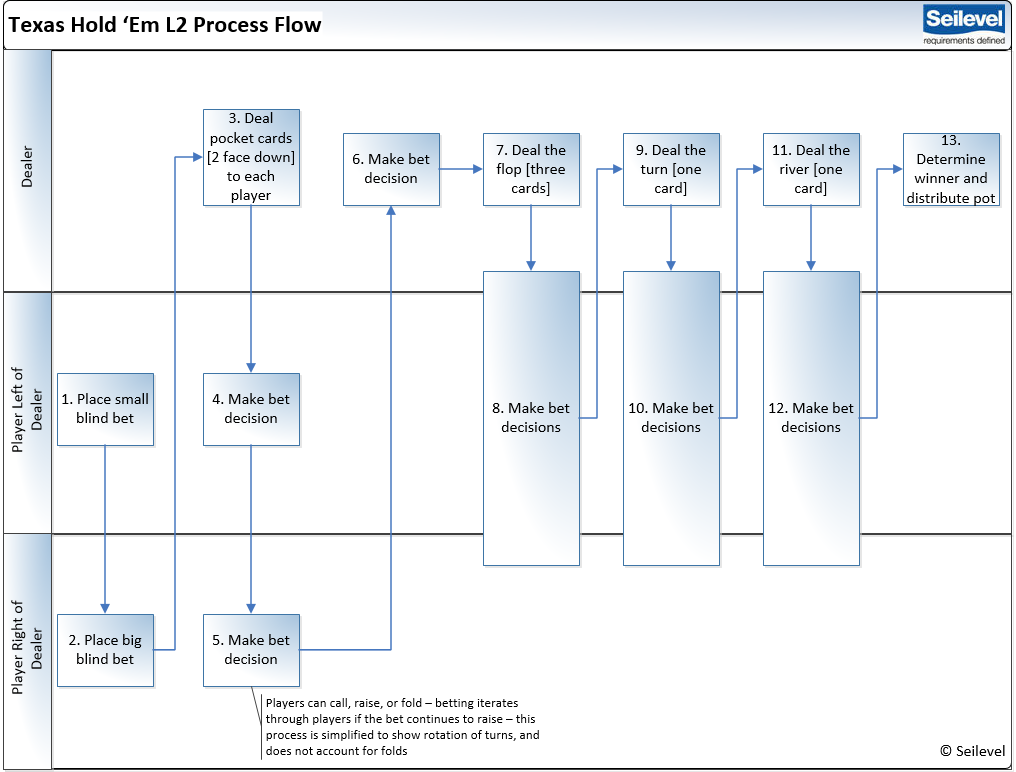
\includegraphics[scale=0.4]{images/process-flow.png}
\caption{Folyamatábra a póker menetéről}
\cite{process-flow}
\label{fig:process-flow}
\end{figure}

\subsection{Alapfogalmak}
Elengedhetetlen, hogy tisztázzunk néhány alapfogalmat. Ezek a következők.
\cite{harrington}
\begin{itemize}
\item Flop: Három kártyalap, ami egyszerre kerül az asztalra, színével fölfelé. Ezek a lapok a játékosok közös lapjai. A flop után egy újabb licitkör következik.
\item Gomb vagy osztó (Button): A kis vak jobb oldalán ülő játékos. A flop után ő kerül utoljára sorra minden licitkörben. A gombot egy fehér korong jelzi, ami az óramutató járásával megegyező irányban körbejár az asztalon.
\item Jó (Out): Olyan lap(ok), mellyek kezünk nyerővé alakulna.
\item Kezdeti bank (Initial pot): A vaktét és az esetleges alaptétek összege a licitálás megkezdése előtt.
\item Kis vaktét (Small blind): Az osztó bal oldalán ölő játékos által a licitsorozat megkezdéseként kötelezően betett tét.
\item Nagy vaktét (Big blins): A kis vak bal oldalán ölő játékos által kötelezően betett tét, a további akciók motiválására.
\item Turn: A negyedik közös lap, ami színével fölfelé az asztal közepére kerül. A turn után újabb licitkör következik.
\item River: Az ötödik és egyben utolsó közös lap, ami az asztal közepére kerül színével fölfelé. A river után az utolsó licitkör következik.
\item Saját lapok (Hole cards): Az egyes játékosoknak a parti elején színével lefelé kiosztott két-két kártyalap. Ezeket a lapokat a többi játékos nem láthatja.
\item Kéz: Egy játékos által, a lent lévő és a kezében lévő lapok közül kiválasztott öt lap.
\item Nuts: A lehető legjobb kombinációval rendelkező játékos keze.
\item Zsetonkészlet (Stack): Egy adott játékos előtt az asztalon lévő zsetonmennyiség.
\end{itemize}

\subsection{Piackutatás}
Mielőtt belekezdtem volna az alkalmazás elkészítésébe, végeztem egy kis piackutatást, milyen platformok/programok vannak, amik a témával foglalkoznak.

Nem kellett messzire mennem, hogy az elsőre rábukkanjak, hiszem a póker közvetítéseken láthatjuk, hogy ki van írva a játékosok nyerési esélye, egy-egy leosztásnál. Ott viszont a program ismeri a játékban lévő játékosok lapjait, valamint az asztalon lévő lapokat. Így könnyebb meghatározni melyik játékos nyer, vagy legalábbis kevesebb számítást igényel. Esetemben az alkalmazás csak a saját lapomat, valamint az asztalon lévőket ismeri.

Létezik egy technika a témával kapcsolatban, amivel a profi póker játékosok az esélyeiket számolják. A lényege csupán annyi, hogy kiszámolják a lehetséges out-okat, amivel javul a kezük, ezeket megszorozzák kettővel, majd annyival, ahány lapra még várunk. Flop esetén kettővel, turn esetén egyel. Így kapnak egy számot, ami ha nagyobb, mint a banki esélyük, akkor matematikailag, vagy éppen gazdaságilag kifizetődő tartani a tétet. Ezzel a megoldással szemben az én elképzelésem alapján nem csak egy közelítő értéket fogunk kapni, hanem specifikusan minden lehetséges leosztásra egy pontos értéket kapunk, emellett még más adatokat is, melyek segítenek eldönteni a felhasználónak mi legyen a következő lépés.

Az interneten két hasonló programot találtam a póker esélyek számítására, mindkettő webalkalmazás és külalakra hasonlítanak az én elképzelésemre. Az elsőnél csak úgy lehet használni az alkalmazást, ha legalább két játékosnak megadjuk a lapjait. Ezzel a probléma ugyan csak az, mint a fent említett televíziós közvetítéseknél ismert megoldással. Ezt az alkalmazást a chardchat.com weboldalon találtam, ami a világ elsőszámú pókeres online közössége.

\begin{figure}[h!]
\centering
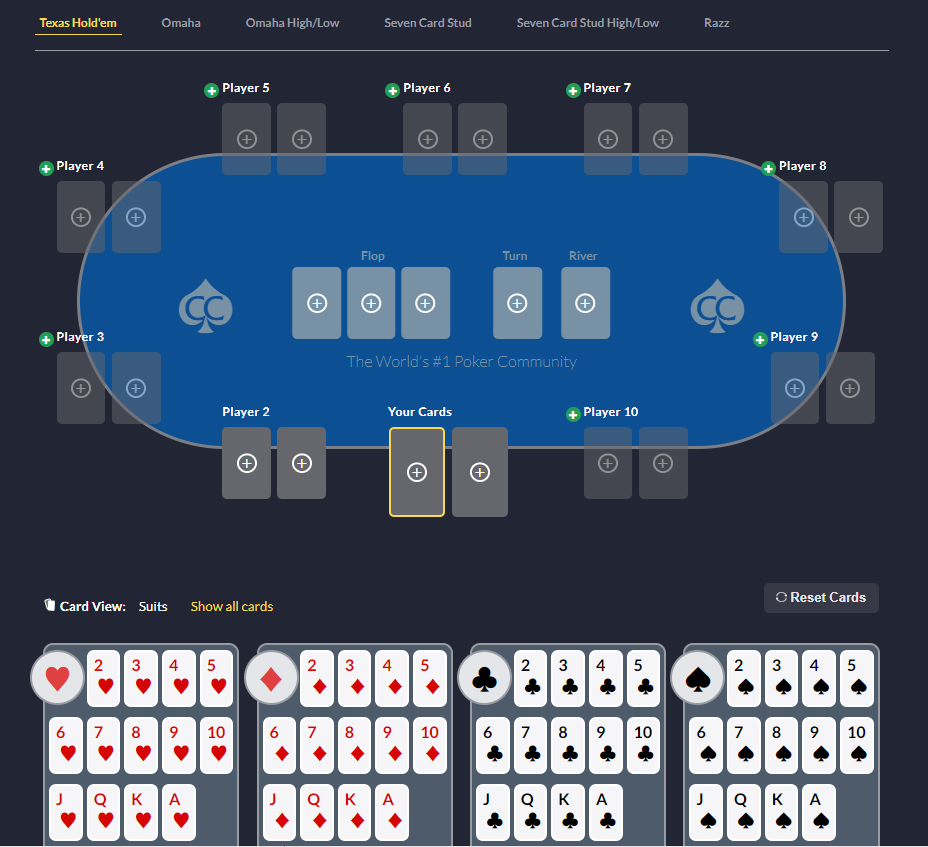
\includegraphics[scale=0.6]{images/cardschat.png}
\caption{Cardschat Poker Odds Calculator}
\label{fig:cardschat}
\end{figure}

A másik szoftver, ami talán a legjobban megközelíti a megoldásomat, a pokernews.com oldalán lévő webalkalmazás. Érdekesség, hogy ezt szintúgy egy óriás, pókerrel foglalkozó cég szponzorálta. A világ talán leghíresebb online póker platformja, a legnagyobb póker versenyek rendezője, a PokerStars. Ebben az esetben tudunk esélyeket számolni úgy is, hogy csak egy játékost választunk ki, csak úgy, mint az én megoldásomnál. Le tudunk rakni 1 és 9 között tetszőleges számú játékosokat, az alkalmazás pedig ezt figyelembe véve számolja az esélyeket. Ezen felül még további esélyeket is látunk, hogy hány százalék a valószínűsége annak, hogy párunk, drillünk, pókerünk, stb. alakuljon ki. Ez a megoldás nagy részben lefedi az általám kigondolt megvalósítást. A különbség, hogy én csak azt szeretném látni, hogy mennyi az esélyem a nyerésre. Az, hogy különböző kezek milyen esélyben alakulnak ki, számomra lényegtelen. Ezzel szemben olyan matematikai mutatók, mint az átlag, a medián vagy a relatív gyakoriság sokkal fontosabb tudni, hogy segítsen a felhasználónak bemutatni az esélyeit.
\begin{figure}[h!]
\centering
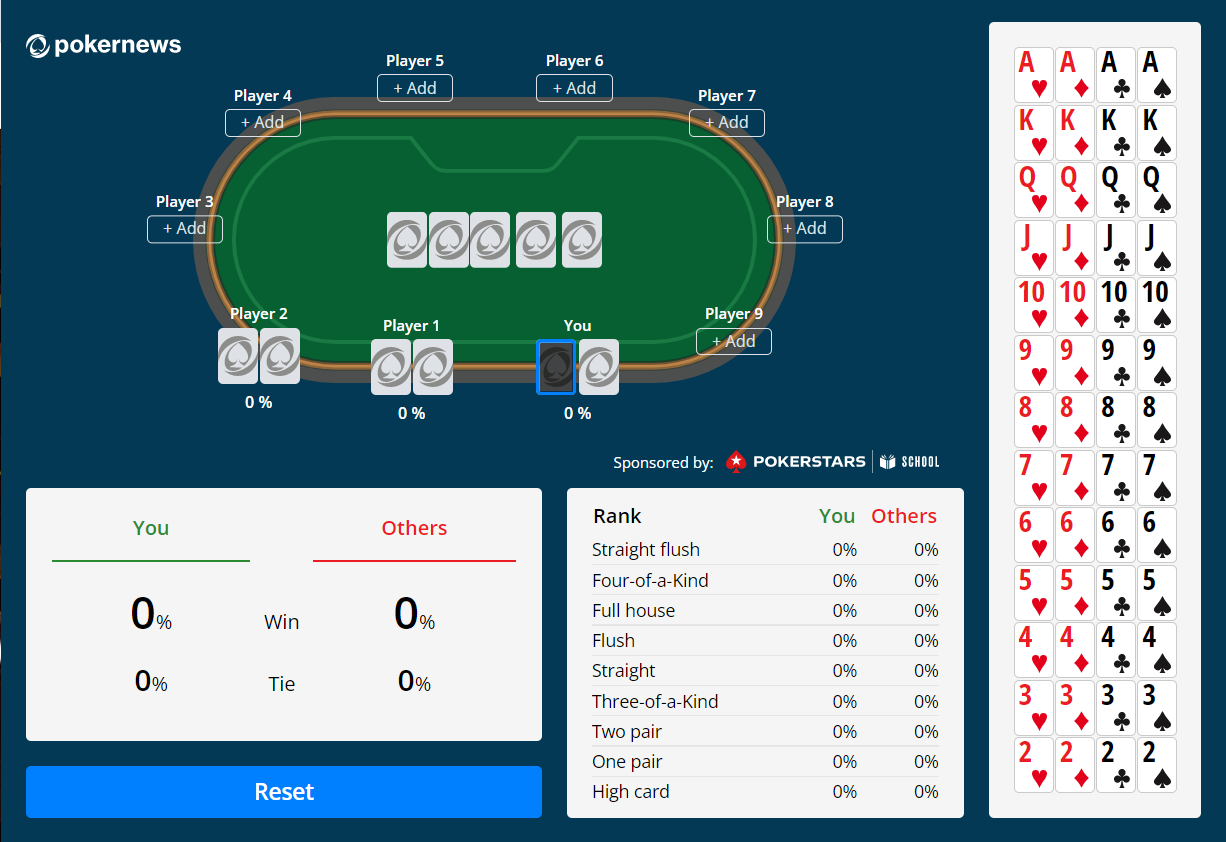
\includegraphics[scale=0.5]{images/pokerstars.png}
\caption{Pokerstars Texas Hold'Em Poker Odds Calculator}
\label{fig:pokerstars}
\end{figure}

\cite{cardschat}
\cite{pokerstars}
\cite{harrington} %hivatkozások mehetnek az utolsó mondat még. Ne álljanak külön 

\Section{Felhasznált technológiák}
Ebben a szakaszban bemutatom az összes olyan technológiát, programozási nyelvet, keretrendszert vagy könyvtárat, amit felhasználtan a szakdolgozatom elkészítése során. Törekszem a tömör magyarázatra. Mindegyiknél próbálom elmagyarázni miért választottam, valamint mik az előnyei, amik számomra kedvezőek voltak.

\subsection{Egyoldalas webalkalmazások}

Ha figyelemmel követjük a Javascript keretrendszerek fejlődését, akkor láthatjuk, hogy egyre nagyobb teret kapnak az egyoldalas alkalmazások (Single Page Application), az olyan többoldalas alkalmazásokkal (Multi Page Application) szemben, mint a jQuery vagy a Laravel.

Három elterjedt Javascript keretrendszert különböztetünk meg. A Facebook által fejlesztett React-ot, az Angulart, amit a Google hozott létre és az Evan You alkotott Vue JS-t.
\cite{vue}

\subsection{Vue JS}

Mindhárom SPA-nak megvan a maga előnye és hátránya. Ezek közül inkább csak a Vue előnyeire koncentrálok a másik kettővel szemben. A három közül ez a legkönnyebben tanulható. Használatához nem szükséges különösebb meglévő Javascript tudás, enélkül is könnyen el lehet sajátítani.

A maga 18 KB-os méretével rendkívül kicsinek számít, amit könnyű letölteni és feltelepíteni, ennek ellenére pozitívan hat a felhasználói élményre és jó keresőmotor optimalizálással is rendelkezik. Saját virtuális DOM-ot (Document Object Model) renderel, ami jobban teljesít mint a React vagy az Angular. Könnyen olvasható a kódja, könnyen integrálható, jól dokumentált, és ezen kívül sok más előnye is van.

Többek között a Vue JS egyik fő tulajdonsága - ami megvan a többi SPA-ban is - hogy komponensekből épül fel, amiket újra felhasználhatunk, ezzel is elősegíti a rövidebb programkódot, átláthatóságot, egyszerűséget, amiket már fent említettem.

Ezek miatt esett a választásom a Vue JS-re, amire több forrás keretrendszerként, mások pedig könyvtárként hivatkoznak
\cite{vue}. %hivatkozást a mondatba rakunk. Ott ahol hivatkoztunk rá. lásd előző mondtat. 

\subsection{Node JS és az Express}

Amellett, hogy a legnépszerűbb programozási nyelv, a Javascript az egyik leginkább univerzális szoftverfejlesztési technológia. Hagyományosan frontend fejlesztésre használták, viszont az utóbbi időben elterjedt a szerver oldali (backend) használata is. Az egyik eszköz - és talán a legismertebb - ami ezt az elmozdulást elősegítette az a Node JS.

A Node JS tulajdonképpen nem egy keretrendszer, nem is egy könyvtár, hanem egy futtató környezet, ami a Chrome V8-as motorján alapszik. A technológiát először 2009-ben mutata be Ryan Dahl az Európai Javascript Konferencián. Amellett, hogy ezen a konferencián rögtön elnyerte a legizgalmasabb szoftver díjat, nem volt használatos széles körben. A technológia 2017-ben csúcsosodott ki, amikor is először használta egy ismertebb cég, a LinkedIn, vagy, hogy még egy párat említsek, a Netflix, eBay és az Uber.

Az egyik hatalmas előnye a Node JS használatának, hogy autómatikusan teljeskörű (full stack) web fejlesztővé válunk vele. Gondoljunk csak bele, két legyet ütünk egy csapásra. Egyszerűen nincs alternatívája a szerver oldali programozásnak a Javascript-ben, csak a Node JS, ez teszi megkerülhetetlenné a technológiát.

Ezek mellett gyors feldolgozású, mivel közös nyelvet használ a frontend és a backend, így a szinkronizáció gyors. Esemény alapú modell-t (event-based model) használ, ezért népszerű választás online játékok, vagy videó konferenciák készítéséhez. Gazdag az ökoszisztémája, az npm - ami a Node JS alapértelmezett csomagkezelője - paranccsal több, mint 800 ezer könyvtárat érhetünk el. Ezen felül több, számos előnye is van, amikre nem térek ki.

Az Express a legnépszerőbb Node JS keretrendszer. Köztes szoftverként (middleware) hivatkoznak rá, amely annyit tesz, hogy tulajdonképpen a kliens és a szerver oldal közötti híd felépítéséhez biztosít eszközöket. Könnyű, rugalmas és véleménymentes keretrendszer. Véleménymentes, mert semmilyen módon nem korlátozza a fejlesztőt, így nagy szabadságot ad. Emellett nagy teljesítményű és hatalmas közössége van a sok felhasználó miatt.
\cite{node}

\subsection{Chart JS}
A Chart JS egy nyílt forráskódú javascript könyvtár adatok megjelenítésére, amely nyolc féle diagramm típust támogat. 2013-ban fejlesztették, mára a második legnépszerűbb diagram készítő javascript könyvtár a GitHub-on. Meglepően egyszerű használni, ez volt a fő oka, amiért ezt választottam. 

A Chart JS HTML5-be renderel. Az én célomhoz csupán két féle diagram típust kell használnom. Az oszlopdiagramot és a vonaldiagramot, ezeket kell egybefűznöm és úgy megjelenítenem.
\cite{chartjs}

\subsection{HTML}
A HTML-ről (Hypertext Markup Language) nem szeretnék hosszasan írni. Talán egy laikus is tudja, hogy ha webalkalmazásról van szó, vagy akár csak egy honlapról, akkor megkerülhetetlen a HTML.

A HTML-t weboldalak készítésére hozták létre, amit később bárki elérhet, aki rendelkezik internet kapcsolattal (feltéve, hogy fel van töltve a weboldal egy domain-re). Használhatunk benne főcímeket, paragrafusokat, beépített képeket, videókat. Ezeket úgynevezett tag-ek határoznak meg. Az elején a kezdő tag, a végén pedig a záró tag.

Szakdolgozatomban a HTML5-öt használtam, amit 2014-ben mutattak be. Többek között olyan újításokat tartalmazott, mint a beépített audio és video tartalom.
\cite{web}

\subsection{CSS}

A CSS (Cascading Style Sheets) egy stílusleíró nyelv. Alkalmazása a HTML elemek kinézetére irányul, azaz hogyan szeretnénk láttatni a weboldalunkon megjelenő tartalmakat.

A CSS a HTML elemekre hat, a kommunikálás pedig többek között a selector-ok segítségével történik. Ezeket a CSS alapból tartalmazza, hivatkozhatunk egy megformálni kívánt paragrafusra, főcímre, valamint megadhatunk saját osztályokat is, amiket többször fel tudunk használni. A deklaráció tulajdonságokat és értékeket tartalmaz.

Itt szeretnék megemlíteni két dolgot, amit a szakdolgozatom készítése során tapasztaltam. Az egyik, hogy érdekes volt számomra megfigyelni, hogy leginkább ez a rész volt az, ami felkeltette az érdeklődésem, ebben tudtam maximálisan kiteljesedni. A másik pedig, hogy megjegyezném az egyre elterjedtebb felhasználási módját a CSS-nek. Ez pedig nem más, mint a Bootstrap, amit azért hoztak létre, hogy könnyedén készítsünk reszponzív weboldalakat, azaz minden képernyőméreten szépen megjelenő oldalakat.

Esetemben tudtam, hogy az én alkalmazásomat számítógép képernyőjén, esetleg más eszközökön, de kizárólag fektetett állapotban lehet használni. Éppen ezért nem láttam értelmét mélyebben beleásni magam ebbe a világba.
\cite{web}

\subsection{Google Firebase}
A Firebase egy szoftverfejlesztő platform, ami 2011-ben indult és 2014-ben került a Google tulajdonába. Valósidejű adatbázisként (Realtime Database) indult, mostanra viszont 18 szolgáltatása és dedikált API-ja (Application Programming Interface) van. Az egész platform egy úgynevezett Backend-as-a-Service megoldást kínál mobil és webalapú alkalmazásokhoz, amely szolgáltatást tartalmaz az alkalmazások fejlesztésére, tesztelésére és kezelésére. 

Számomra a legfőbb előnyei a technológiának, amiért ezt választottam a következők. Teljesen ingyenesen lehet használni a legtöbb szolgáltatását. Könnyű hozzáférést biztosít az adatokhoz, a Firbease console-on keresztül. Könnyő az integrálása is és minimális programozási ismereteket kíván, tehát majdnem, hogy bárki be tudja építeni az alkalmazásába.

Annak ellenére, hogy ez egy nagyon összetett paltform, az alkalmazásom kizárólag a Real Time Database-t használja ezekből. A Google Firebase végzi az autencikációt, vagyis a regisztrációt és a bejelentkezést az oldalra.
\cite{firebase}

\subsection{JSON}
A JSON (Javascript Object Notation) egy szövegalapú nyílt szabvány, amit emberek számára is könnyen olvasható adatátvitelre terveztek. Javascript alapú alkalmazásokhoz, valamint hálózati kapcsolaton keresztüli továbbításra használják. 

Egyik és talán legfontosabb előnye, hogy a legtöbb script nyelvben közvetlenül megfelel az alapvető adattípusoknak, továbbá különbséget tesz a string, number és boolean értékek között. Tehát könnyedén lehet használni a webfejlesztés során. 

Objektumokat hozhatunk benne létre, melyekre kulcsokkal tudunk hivatkozni. Számomra ez volt a fő szempont, mert nagy adathalmazzal kell dolgoznom és ezekben keresést végezni, ami ezzel a módszerrel gyorsnak tekinthető.

\Section{Tervezés}

\subsection{Az alkalmazás megjelenítése}
Az alapvető elképzelésem az alkalmazás külsejéről az volt, hogy az oldalra érkezéskor rögtön egy autentikációs felület fogadja a felhasználót. Ezzel egy amolyan privát jelleget szerettem volna kölcsönözni az egésznek, hogy csak az használhassa, aki regisztrált. A regisztráció/bejelentkezés után egy főoldal fogad minket. Ezen az oldalon a Texas Hold'Em póker változatról egy rövid leírást mutatok be, valamint az alkalmazás lényegét szemléltetem. Az oldal tetején van egy egyszerű navigácóis felület, ahol tovább mehetünk arra az oldalra, ahol magát a játékot találjuk.

Itt is az egyszrűséget tartom szem előtt. Középen helyezkedik el egy pókerasztal felülnézetből. Alatta jelenítem meg a négy színt (treff, káró, kör, pikk). Ezekre rákattintva előjön az adott színből az összes (13) kártya, ami közül kiválasztunk először egyet, ez a lap pedig eltűnik a választható lehetőségek közül és lekerül az asztalra saját lapként. Megint a négy színt látjuk, amiből ismét kiválasztunk egyet, és még egy lapot. Ezek után ugyan ezzel a módszerrel tudjuk lehelyezni az asztal közepére is a közös lapokat.

Minden licitkör előtt az asztal mellett láthatja a felhasználó az összesített nyerési esélyét, ami segít neki a döntés meghozásában. Ha több lapot szeretne a felhasználó az asztalra tenni mint a 2 (saját) + 5 (közös), akkor egy pop up ablak ugrik fel, ami jelzi neki, hogy már több lapot nem használhat. Két választása van ebben az esetben, az egyik, hogy figyelmen kívül hagyja, ilyenkor elemezheti tovább az esélyeket. A másik, hogy új leosztást kezd, ilyenkor eltűnik minden lap az asztalról és folytathatja a játékot.

\subsection{Alapötlet} % Jól megírtad és átadtad a lényeget. 
A tervezés első lépése a módszer meghatározása volt, amellyel az esélyeket számoljuk. Ezt hátulról előre haladva közelítettem meg, azaz a rivernél kezdtem, a turn-ön át, egészet a preflopig. Ennek oka az volt, hogy a legkevesebb számítás akkor van, amikor minden lap lent van és tudjuk, hogy nekünk milyen erős kezünk van, így azzal ebben az esetben nem kell folglakozni, tehát bonyolultsági sorrendben haladtam.

Az alapötlet az volt, hogy legenerálom az összes lehetséges 7 lap együttesét, amelyekhez egy értéket rendelek, hogy mennyire erősek. Természetesen a legerősebb a royal flush, a leggyengébb pedig a 7-es magaslap. Csak, hogy szemléltessem a számolások bonyolultságát és nagyságát, ez \[ \binom{52}{7}=133.784.560\] eset. Turn esetében ismerem az én 7 lapomat, tehát csak egy keresést kell végezni ebben az adathalmazban, ami visszatér a kezem értékével. Az ellenfél esélyeinek kiszámítása már egy kicsit komplikáltabb. Az 52 lapból ismerünk 7-et, tehát a pakliban 45 lap marad. Ebből választhat további 2 lapot az ellenfél, ez \[ \binom{45}{2}=990\] lehetőség az ellenfél kezeire. Ez a szám fontos szerepet játszik a dolgozat történetében, és végig jelen lesz a dokumentációban. Erre a 990 lehetőségre mind el kell végezni a keresést a kb. 133 milliós adathalmazban, így kapunk 990 értéket. Innentől kezdve már csak az a dolgunk, hogy hány százalékban kissebb a mi kezünk értéke az ellenfél lehetséges kezeinél. 

Tovább haladva a turn esetében vizsgáljuk az esélyeket, amikor is csak 4 lap van az asztalon, egy lapra pedig még várunk, ami egyelőre ismeretlen. Itt kissé bonyolultabb a helyzet, mivel a saját kezünk értékét sem ismerjük. Természetesen vannak szélsőséges esetek, mikor már a turn-nél pókerünk vagy royal flush-ünk alakul ki, ezekben az esetekben nem releváns az utolsó lap, mindenképp nyertünk. Ilyen esetek azonban ritkán fordulnak elő. Először ki kell számolnunk a saját esélyeinket, amit majd össze tudunk hasonlítani az ellenfél esélyeivel. Két lap a kezünkben, négy lap az asztalon, 46 lap maradt, ami érkezhet az asztalra utolsóként. Mind a 46 lapra meg kell keresnünk az adathalmazban a kezünk értékét, így a saját kezeinkre lesz 46 értékünk. Ezután mind a 46 lehetséges utolsó lapra meg kell keresnünk az ellenfél 990 lehetséges kezére az értékeket, ez 45.540 eset. Amint ezek megvannak, össze tudjuk hasonlítani az értékeket.

A flop esetében lévő értékek számításánál még több számítást kell végeznünk. A saját két lapunkon kívül itt már csak három lent lévő lapot ismerünk. Ez azt jelenti, hogy turn-re jöhet 47 féle lap, river-re pedig további 46 féle. A saját lapjaink \[ \binom{47}{2}=1081\] féle képpen jöhetnek le. Ezek alapján az ellenfélnek \[1081\cdot990=1.070.190\] lehetséges keze van. Ezekre a lehetséges kombinációkra mind keresést kell végeznünk az adathalmazban, hogy megkapjuk a saját és az ellenfél értékeit, amivel tovább tudunk dolgozni.

<<<<<<< Updated upstream
Az utolsó licitkör, aminél számításokat kell végeznünk, az tulajdonképpen a játék menetét illetően az első licitkör. A preflop esetben nem ismerünk semmilyen lapot, csak azt a kettőt, amit osztottak nekünk. Az 52 lapos pakliból 50 lap érkezhet az asztalon lévő első helyre, a másodikra 49, az ötödikre, vagyis az utolsóra pedig 46 lehetséges lap. Itt kell a legtöbb számítást végezni, amikor is \[ \binom{50}{5}=2,118,760\] különbözőképpen alakulhat ki a saját kezünk. Ezt megszorozva a már ismert rivern-nél lévő ellenfél kezeinek kombinációjával, az ellenfél lehetséges kezeinek száma 2.097.572.400, ami több, mint két milliárd eset. Ennyi értékkel kell majd számolnunk a továbbiakban. Ez jól mutatja, hogy milyen összetett a problémakör és, hogy mennyi számítást igényel. Az alapötletben ezt nem számoljuk valós időben, hiszen rengeteg időt venne igénybe. Ehelyett egyszer legeneráljuk ezeket a kombinációkat az összes lehetséges kézre preflop, ami 1326 lehetőség, tehát ennyivel kell megszoroznunk még a fent említett számot.
=======
Az utolsó licitkör, aminél számításokat kell végeznünk, az tulajdonképpen a játék menetét illetően az első licitkör. A preflop esetben nem ismerünk semmilyen lapot, csak azt a kettőt, amit osztottak nekünk. Az 52 lapos pakliból 50 lap érkezhet az asztalon lévő első helyre, a másodikra 49, az ötödikre, vagyis az utolsóra pedig 46 lehetséges lap. Itt kell a legtöbb számítást végezni, amikor is \[ \binom{50}{5}=2,118,760\] %valahol vesszőt valahol pontot, valahol semmit nem használsz a helyiérték jelölésére. Légy konziztens! 
különbözőképpen alakulhat ki a saját kezünk. Ezt megszorozva a már ismert rivern-nél lévő ellenfél kezeinek kombinációjával, az ellenfél lehetséges kezeinek száma \linebreak 2.097,572.400, ami több, mint két milliárd eset. Ennyi értékkel kell majd számolnunk a továbbiakban. Ez jól mutatja, hogy milyen összetett a problémakör és, hogy mennyi számítást igényel. Az alapötletben ezt nem számoljuk valós időben, hiszen rengeteg időt venne igénybe. Ehelyett egyszer legeneráljuk ezeket a kombinációkat az összes lehetséges kézre preflop, ami 1326 lehetőség, tehát ennyivel kell megszoroznunk még a fent említett számot.
>>>>>>> Stashed changes

\subsection{Esélyek vizsgálata}
A piackutatás során derült fény számomra arra, hogy a legtöbb ehhez hasonló alkalmazás csak egy átfogó százalékos esélyt adott az éppen aktuális leosztásról. Ez volt az egyik motivációm arra, hogy az én alkalmazásom ennél többet adjon a felhasználónak.

Azon kívül, hogy egy összefogó százalékos esélyt számítok minden licitkörnél, létrehozok egy oszlopdiagrammot is, amelyben minden lehetséges következő lap(ok)ra kirajzolom, hogy annál a losztásnál milyen százalékban nyer a felhasználó. Rivernél ennek nincs sok jelentőssége, mivel ismerjük az összes lapot. Itt csak két oszlop lesz, az én, illetve az ellenfél nyerési esélye. Turn-nél 46 lap érkezhet még, így 46 oszlopunk lesz, aminél láthatjuk, hogy melyik esetben mennyi esélyünk van nyerni, ezek mellett természetesen az összesített esélyt is megjelenítem. Erre azért van szükség, hogy tisztább képet nyújtsak a felhasználó számára az esélyeiről. Egy példán keresztül megvilágítva, lehet, hogy a turn-ön 70\% esélyünk van a nyerésre, viszont ha ez úgy adódik össze, hogy 9 esetben 100\% az esélyünk, 11 esetben 90\%, 6 esetben 80\%, a maradék 20 esetben pedig 40\%, akkor jobban át kell gondolnunk a következő lépésünket, mintha ez a 70\% egymáshoz közel álló számokból alakulna ki.

Emellett, a diagrammon több konstans értéket is megjelenítek. A fent említett oszlopdiagramm sokat segít a döntés meghozásában, viszont nehezen elemezhető. Éppen ezért szemléltetem az ellenfél nyerési esélyének az átlagát, a mediánját, valamint a szórását is. Ezek további segítséget nyújtanak a felhasználónak.

A diagram alatt található egy beviteli mező, ahova egy számot adhatunk meg. Itt számolja az alkalmazás a realtív gyakoriságot, vagy más néven az empirikus valószínűséget. Tulajdonképpen az ide beütött érték előfordulásának számát kapjuk meg. Ha kiváncsiak vagyunk arra, hogy az ellenfélnek mennyi esetben van több esélye nyerni, mint 50\%, akkor beütjük azt, hogy 50 és ki fogja írni a relatív gyakoriságot. Ez az érték 0 és 1 közé eshet.
\Chapter{Technikai kivitelezés}
Ebben a fejezeetben bemutatom az elkészült programot a számomra legérdekesebb programrészletekkel. Nem térek ki minden funkcióra és programkódra, csak a lényegesebb egységekre. Részletezem a front end kivitelezését, amelybe tartozik a Vue JS, HTML és CSS kódok. Ezután a back end számításokat mutatom be, amelyet Node JS környezetben valósítottam meg.

\section{A projekt felépítése}
Mielőtt belekezdek a megoldásaim, függvények, programkódok magyarázásába, először bemutatom a projekt felépítését, hogy egyszerűbben érthető legyen. Először a webalkalmazás felépítését mutatom be. 

A webalkalmazás frontend részét a már említett Vue JS-ben valósítottam meg. Ebben vannak a komponensek és a vue-router, amely az oldalak közti mozgást végzi el. A front end és a back end közötti kommunikációt az API végzi. A JSON adatbázis lokálisan helyezkedik el és csak a back end kommunikál vele, illetve használja a számításokhoz.

\begin{figure}[h]
\centering
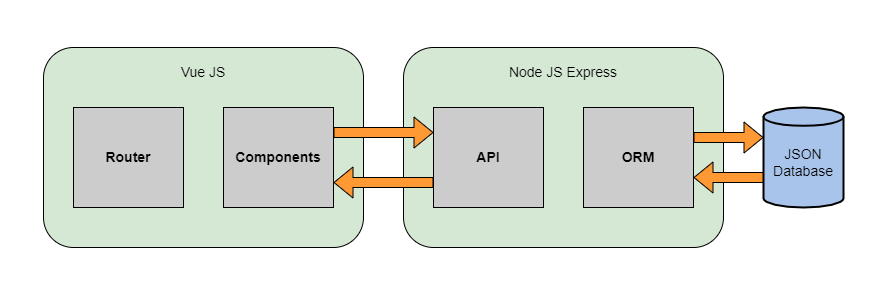
\includegraphics[scale=0.8]{images/web-arch.png}
\caption{A webalkalmazás architektúrális ábrája}
\label{fig:web-arch}
\end{figure}

A 3.2-es ábrán látható az elkészült projekt struktúrája file rendszer szinten. Az ábra bal oldalán a front end látható felépítése látható. A components mappában vannak a komponensek, amelyeket többször fel lehet használni az oldalakon. 

A router mappában lévő index.js file-ban vannak definiálva a router-ek. Itt meg kell adni az elérési útvonalat, az oldal nevét, amelyre irányítani szeretnénk a felhasználót, illetve importálni az adott vue file-t. Ezeket az oldalakat a views mappában találjuk, itt az autentikációt végző oldalak, a home fül és a SimulateGame helyezkedik el, amelyben maga a póker alkalmazás valósul meg.

Ezeken kívül a main.js-ben importálni kell minden olyan kiegészítőt, melyet használok az alkalmazásban, valamint a Firebase config része is itt van definiálva. Fontosak még az css file-ok, ezeket importálom be az egyes oldalakon, hogy a megfelelő megjelenést kölcsönözzem nekik. Ezeken kívül a package.json és package-lock.json file-okban meg vannak adva a felhasznált technológiák verziója, hogy ne legyen köztük ütközés.

Az ábra jobb oldalán látható az alkalmazás back end része. Itt az erchitektúra jóval egyszerűbb. Két json adathalmazt hoztam létre, az egyik a kártyák erősségét tárolja, a másik a preflop esélyeket, mind a kettőbe egy-egy objektum helyezkedik el. Itt is megtalálható a package.json és a package-lock.json, ezek ugyan azt a szerepet töltik be, mint a front end-nél. Az index.js is hasonló mint a front end-en, itt is be kell importálni minden felhasznált technológiát, valamint megadni, hogy milyen porton fusson a back end. Erre azért van szükség, hogy a localhost-on futtatott kliens és szerver ne kavarodjon össze.

A findStrongest.js-ben azok a kódok vannak, melyek a felhasználó esélyeit vizsgálja, a findEnemyStrongest.js-ben pedig azok, amik az ellenfél esélyeit. A helperFunctions.js arra szolgál, hogy a több helyen meghívott függvényeket eltárolja, így azokat nem kell többször megírni. Végül a root.js-ben két post response helyezkedik el, így történik az adatátvitel a kliens részére.

\begin{figure}[h]
\centering
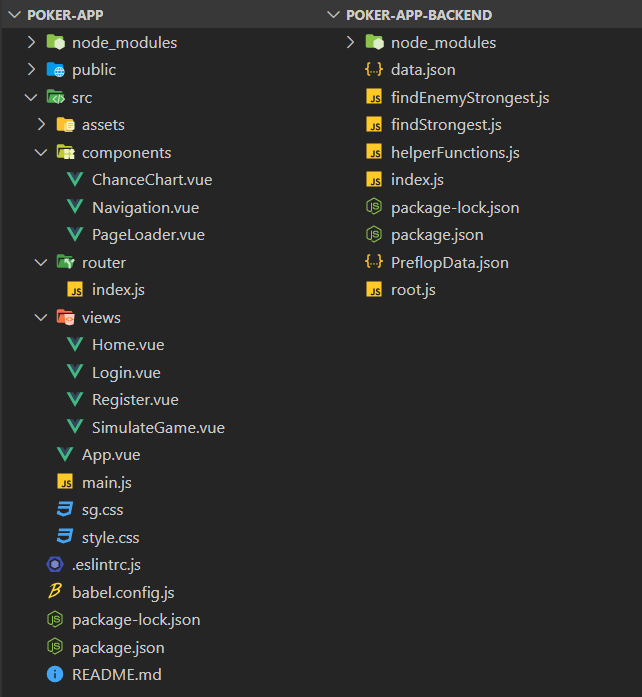
\includegraphics[scale=0.8]{images/frontend-backend-arch.png}
\caption{A projekt struktúrája file rendszer szinten}
\label{fig:frontend-backend-arch}
\end{figure}

Az osztály diagrammon bemutatom, hogy nagy vonalakban milyen adatokkal, fügvényekkel és a hozzájuk kapcsolódó paraméterlistákkal dolgoztam. Ez a 3.3-as ábrán látható. A kék elem a klienst szemlélteti, a sárgák pedig a szervert hivatottak megvalósítani.

Az adatok mindenhol tartalmazzák a sevenCards és az everyCards adatokat, kivéve a helperFunctions-nál, hiszen onnan csak meghívom a függvényeket. A front end oldalon továbbá jelen van a myCards is, erre az esélyek ábrázolása miatt van szükség. Itt jelenítem meg a diagramokat a chartCalc függvénnyel. A chooseCard függvény veszi ki a lapokat a pakliból, amit majd továbbadok a szervernek, valamint a lapok megjelenítésében is szerepet játszik. A két backend függvény pedig két post request-et tartalmaz.

A sárga részeken találhatóak azok az adatok és függvények, amik az esélyek számolásáért felelősek. A teljesség igénye nélkül, itt számolom a lehetséges érkező lapokat, ezekre az értékeket, sorba rendezem a lapokat, leszűkítem a csak a nevekre, és egyéb lent látható eseményeket.

\begin{figure}[h]
\centering
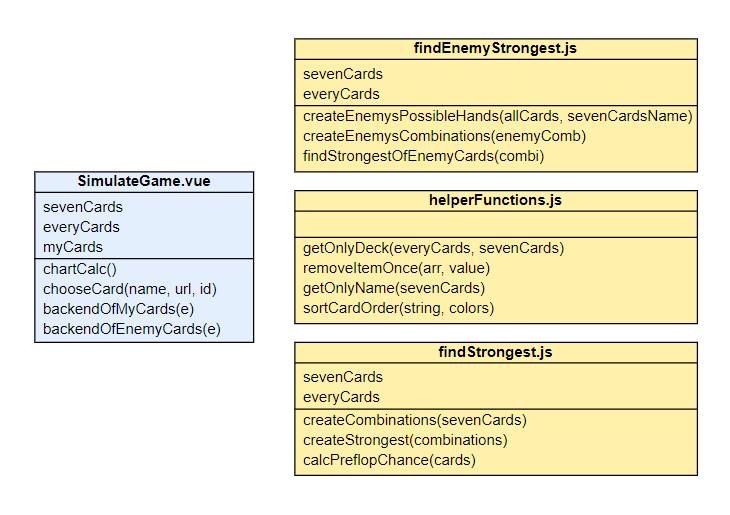
\includegraphics[scale=0.9]{images/class-model.png}
\caption{Az alkalmazás osztály diagrammja}
\label{fig:class-model}
\end{figure}

\section{Front end kivitelezése}
Egy webalkalmazás front end része az, amit a felhasználó érzékel az oldalról. Itt részletesen bemutatom a főbb egységeket, melyek Vue JS-ben íródtak. A HTML és CSS részekre csak minimálisan térek ki, itt pedig igyekszem azokat a megoldásokat bemutatni, melyek a legizgalmasabbak voltak a kivitelezés során. 

\subsection{Autentikáció}
Az alkalmazás első oldala a bejelentkező/regisztrációs felület. A két oldal kissebb eltérések mellett ugyan az, ezért nem térek ki külön csak a változásokra. A register oldalon meg kell adnunk egy e-mail címet, egy hozzá tartozó jelszót, valamint egy becenevet is. Ha regisztráltunk, akkor a login oldalon csak megadjuk az e-mail címünket és a hozzá tartozó jelszót, a sign in gombra kattintunk és már be is enged minket az oldal. A bejelentkezést és a regisztrációt a Firebase végzi, valamint a validációt is. Az e-mail címnek tartalmaznia kell egy kukac jelet, illetve pontot és egy domain-t. A jelszónak legalább hat karakter hosszúnak kell lennie.

Ennek a két oldalnak a HTML része nagyon egyszerű. Egy formot belül két szöveges beviteli mezőt, ezen kívül egy gombot találunk. Mindezt közbezárja egy div, ami tartalmaz még két címet is, melyek a login és a sign up feliratok, ezekkel tudunk váltani a két oldal között. A login rész még kiegészül egy harmadik beviteli mezővel, ami a becenév.

\begin{python}
<div class="login">
  <h2 class="active"> Login </h2>
  <h2 class="nonactive"><router-link to="/register"> Sign up </router-link></h2> 
  <form @submit.prevent="Login">
    <input type="text" class="text" name="E-mail" v-model="email">
    <span>E-mail</span>
    <input type="password" class="text" name="password" v-model="password">
    <span>password</span>
    <button class="signin" value="Login">
      Sign In
    </button>
  </form>
</div>
\end{python}

Az autentikációt viszonylag egyszerű elvégezni a Firebase segítségével. Regisztrációnál a createUserWithEmailAndPassword függvényt használjuk, amivel létrehozunk egy felhasználót. Ehhez egy e-mail cím és egy jelszó tartozik, jelen esetben kieégüszlve egy becenévvel. Ezt el is tárolja nekünk a Firesotre Database-ben.Ezután bejelentkezésnél a signInWithEmailAndPassword függvényt használjuk, amely megkapja az e-mail és jelszó párost, és ha ez egyezik, már bent is vagyunk a főoldalon.

\begin{python}
const Register = () => {
      firebase
        .auth()
        .createUserWithEmailAndPassword(email.value, password.value)
        .then((user) => {
          db.collection("users")
            .doc(user.uid)
            .set({nickname: nickname.value})
        })
        .catch((err) => alert(err.message));
    };
\end{python}

Az autentikációs oldalak stílusa talán a leglátványosabb az alkalmazásban. Igyekeztem egységesen megformázni az összes oldalt. Ahol lehet lekerekítést használok, és mindenhol a azonos kék és piros színekkel kombinálok. A CSS legérdekesebb része számomra ebben a részben a két címsor formázása volt. A felhasználónak ez csupán színek váltakozása, viszont annál sokkal érdekesebb. Mikor melyik cím aktív, úgy annak a színe változik fehérré és kap egy aláhúzást, a másik címsor pedig elhalványodik. Ezt a login és a register oldal váltásával jelenítem meg.

\begin{python}
.active {
  border-bottom: 2px solid #1161ed;
}
.nonactive {
  color: rgba(255, 255, 255, 0.2);
}
\end{python}

\subsection{Főoldal és navigációs fejléc}
A főoldalról nem szeretnék hosszasan írni, mert tartalmilag is elég rövid. Mindössze két block elemben két paragrafus található benne, formázva. Az egyik röviden leírja a póker játék lényegét, a másik pedig megfogalmazza, miről is szól az alkalmazás.

A Vue JS egyik előnye, hogy komponensekből épül fel, melyeket többször fel tudunk használni. Nekem az egyik ilyen komponensem a navigációs fejléc. Ezt mindegyik oldalon felhasználom, hiszen a felhasználó ezen keresztül tud váltani az oldalak között. Másik sajátossága a view-router, ami megvalósítja az oldalak közötti ugrást, ezek az index.js file-ban vannak definiálva.

\begin{python}
<nav class="navbar">
  <ul>
    <li class="stand"><router-link to="/" class="must">Home</router-link></li>
    <li class="stand"><router-link to="/simulategame" class="must">Simulate Game</router-link></li>
    <li @click="Logout" class="log"><router-link to="/login" class="must">Logout</router-link></li>
  </ul>
</nav>
</template>
\end{python}

A Vue-nak köszönhetően ebben a komponensben nincs szükség javascriptre, anélkül tudunk váltani az oldalak között. Természetesen ezt is formázom CSS-el.

\subsection{Játék szimuláció}
Az alkalmazás nagy része front end részről a SimulateGame.vue oldalon van. Itt találjuk magát a játékot. Az oldalra érkezéskor a közepém egy pókerasztalt látunk, alatta pedig a 4 színt. Ezek közül egyre rákattintunk, akkor felugrik abból a színből mind a 13 lap, itt tudunk kiválasztani egyet. Ha ez megtörtént, akkor az a lap eltűnik a választási lehetőségek közül, többször már nem választhatjuk, valamint hozzáadja egy tömbhöz, majd ugyan ezt megismételjük 6-szor. Az összes lapot előre definiáltam. A lapokra való kattintáskor meghívódik a chooseCard() függvény, amely a fentieket végzi el.

\begin{python}
    chooseCard(name, id, url) {
      if (this.isThere === 8) {
        this.cardsFull = true;
        return;
      }
      this.sevenCards.push({ name, url });
      this.isThere = this.isThere + 1;
      this.showPic = false;
      this.isHidden = false;
      this.cards[id - 1] = false;
    }
\end{python}

A függvény elején rögtön egy feltétel van, ami ellenőrzi, hogy ne rakhassunk le 7 lapnál többet az asztalra. Amennyiben így szeretnénk tenni, egy pop up ablak ugrik fel, amely jelzi a felhasználónak, hogy több lapot már nem tehet le.

Ezen kívül a kiválasztott lapot belerakjuk a sevenCards globális objektumba, melyet majd továbbadunk a back end-nek, hogy végezze el a számításokat. Továbbá tartalmaz pár egyéb külső változót is, melyek a színek és lapok megjelenítéséért felelnek.

A másik lényeges rész ezen az oldalon az esélyeket megjelenítő diagram. Ez is egy külön komponens, viszont itt töltöm fel adatokkal. A back end-től megkapjuk az összes következő lapra számolt esélyt. Az ellenfélnek mindig 990-szer több esete lesz, hiszen nem ismerjük a lapjait. Emiatt a mi esélyeink első esetét össze kell hasonlítani az ellenfél eslő 990 esetével, ebből kapunk egy százalékos esélyt, amely majd az első oszlopunk lesz a diagrammon, és így tovább. 

Ezek mellett még olyan matematikai értékeket is számolok, mint az átlag, a medián vagy a szórás, melyek közül szerintem az utóbbi a legérdekesebb.

\begin{python}
        calculateDeviation(arr) {
      let mean =
        arr.reduce((acc, curr) => {
          return acc + curr;
        }, 0) / arr.length;
      arr = arr.map((k) => {
        return (k - mean) ** 2;
      });
      let sum = arr.reduce((acc, curr) => acc + curr, 0);
      return Math.sqrt(sum / arr.length);
    }
\end{python}

A felhasználó továbbá meg tud adni egy értéket is, amelyre az alkalmazás kiszámolja a relatív gyakoriságot, így többlet információhoz juthat, hogy mennyi esetben van például 50\% felett az ellenfél nyerési esélye.

\section{Back end kivitelezése}
A back end rész megvalósítása véleményem szerint a legkiemelkedőbb eleme a szakdolgozatomnak. Itt Node JS programkódok fognak szerepelni a hozzájuk tartozó magyarázattal, valamint bemutatom az adathalmazomat is.

\subsection{Adathalmaz bemutatása}
Úgy gondolom, átláthatóbb a dokumentáció úgy, ha először az adathalmazomat mutatom be, ugyanis erre többször fogok hivatkozni a későbbiekben. 

Mint azt az alapötlet szakaszban is említettem, először egy kb. 133 millió soros adathalmazzal kezdtem el a megvalósítást, melyben az összes lehetséges 7 lap kombinációja benne volt. Ezt pythonban magamnak generáltam le. A generáció futási ideje 7,5 óra volt, az adathalmaz mérete pedig 6 GB.

\begin{python}
from itertools import combinations

cards = combinations(["2c", "3c", "4c", ... , "As"], 7)
sevenCards = {}
sevenCards["cards"] = []

with open("data_new.json", "w") as outfile:
    for c in cards:
        c = list(c)
        outfile.write(f"{c}, \n")
\end{python}

Hamar kiderült, hogy ez akkora adathalmaz, amivel nagyon nehezen tudtam volna a továbbiakban dolgozni. Rengeteg keresést kell végeznem ebben, ami nagyon sok időbe telne, ezért más megoldást kellett találnom.

Az interneten találtam egy másik adathalmazt, amely lényegesen kisebb volt, 7462 soros, ezt használtam fel. 
\cite{chances}
Ez a lehetséges 5 lap kombinációinak száma úgy, hogy nem vizsgálunk külön minden színt. Így a számításaim annyival bővültek, hogy a kiválasztott 7 lapból \[ \binom{7}{5}=21\] keresést kell végeznem, hogy megtaláljam a legerősebb 5 lapot, amit a felhasználó magától is ki tud választani, viszont az alkalmazásnak is tudnia kell, tehát ezzel kell majd tovább számolnia.

Az adathalmazt JSON-ben tároltam el. Egyetlen objektumot tartalmaz, aminek az értéke a kombinációk, a kulcsa pedig a kéz erőssége. Azoknál az eseteknél, ahol számításba kell vennünk, hogy a lapok színe azonos, ott egy F betűt szúrtam az értékekbe. Ezeket abc sorrendbe rendeztem az egyszerűbb felhasználás végett.

\begin{python}
{
  "cardStrenght": {
    "AFJKQT": 1,
    "9FJKQT": 2,
    "89FJQT": 3,
    "789FJT": 4,
    "6789FT": 5,
    .
    .
    .
    "23457": 7462
    }
}
\end{python}

Az első 10 érték a színsorok, royal flush-el kezdve, a 11-dik az ász póker király kísérővel, a 7462-dik pedig a 7-es magaslap.

A projekt vége felé közeledve, a preflop esélyek számolása az addig alkalmazott módszer szerint még mindig túl sok időt vett volna igénybe. Mivel két lap ismeretében nincs is annyi értelme több matematikai értéket szemléltetni, így arra jutottam, hogy csak egy százalékos esélyt fogok mutatni a többi lap ismerete nélkül. Ehhez létrehoztam egy hasonló adathalmazt, mint a kártyerősséget tartalmazó, ezt elneveztem PreflopData.json-nek. A tartalmát az alábbi táblázat adja. A párok alkotta átló fölött lévő kezdőlapok az egyszínűek esélye, alatta pedig a különböző színű lapoké.

\begin{figure}[h]
\centering
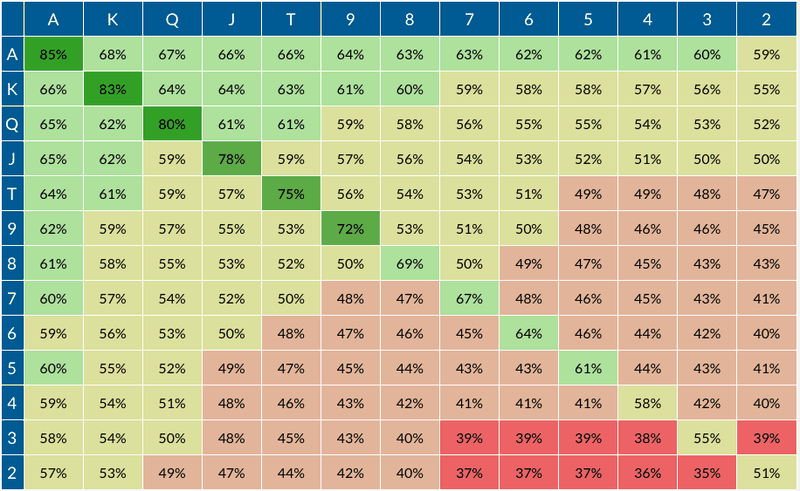
\includegraphics[scale=0.5]{images/preflop-chances.png}
\caption{Preflop kezek esélyei}
\cite{preflop-chances}
\label{fig:preflop-chances}
\end{figure}

\subsection{A felhasználó esélyeinek számítása}
Az egyszerűbb része az esélyek számolásának a felhasználó esélyeinek a kiszámolása, ugyanis itt kevesebbet kell számolni. 

A back end megkapja a front end-től a felhasználó által kiválasztott lapokat. Itt is definiálva van a pakli minden lapja, viszont objektum helyett csak egy tömbbe, mivel csak a lapok nevére van szükségünk. A default függvényben egy ellenőrzést végzek, hogy milyen hosszú az objektum, amit megkap. Erre azért van szükség, mert különböző számításokat kell végezni ha a flop-nál, turn-nél vagy river-nél szeretnénk megtudni esélyeinket. Először minden esetben a getOnlyName és a getJustDeck függvényeket használom. Az előbbivel az objektumot egy tömbre szűkítem, hogy csak a kártyák neveivel dolgozhassak tovább. Az utóbbival az összes lapot tartalmazó tömbből kitörlöm azokat, amelyeket a felhasználó már kiválasztott, így megkapom a pakliban maradt lapokat.

River esetében a tömb hosszúsága 7. Itt van a legegyszerűbb dolgom, mivel minden lap ismert, csak vissza kell térni a felhasználó kezének értékével. Először legenerálom a 7 lapból az összes 5 lap kombinációját, ezt a createCombinations függvénnyel teszem. Ez megkap egy 7 elemű tömbböt és visszatér 21, 5 elemű tömbbel.A generációhoz a javascript generatorics nevű kombinatorikai könyvtárát használom.

\begin{python}
function createCombinations(sevenCards) {
  let allCombinations = [];
  for (let comb of G.combination(sevenCards, 5)) {
    allCombinations.push(comb.slice());
  }
  return allCombinations;
}
\end{python}

Ha megvan a 21, 5 elemű tömbbünk, akkor már csak meg kell keresni mindegyiknek az értékét az adathalmazban, majd kiválasztani a legkissebbet és azzal visszatérni. Ezt a createStorngest függvény valósítja meg, amely megkapja az előbb említett 5 lapos kombinciókat és visszatér a legerősebb 5 lap értékével.

\begin{python}
function createStrongest(combinations){
  let rawdata = fs.readFileSync("data.json");
  let strenghtOrder = JSON.parse(rawdata);
  let result =  [];
  for (let combination of combinations) {
    let nameString = "";
    let colors = { C: 0, S: 0, H: 0, D: 0 };
    for (let card of combination) {
      nameString += card[0];
      colors[card[1]] += 1;
    }
    let ordered = sortCardOrder(nameString, colors);
    result.push(strenghtOrder.cardStrenght[ordered]);
  }
  return Math.min(...result);
}
\end{python}

A strengthOrder változóban eltárolom az adathalmazt. Egy foreach ciklussal végigmegyek mind a 21 kombináción. A cikluson belül ellenőrzöm, hogy a lapok között hány egyforma színű lap van, hiszen ha mind az 5 egyforma színű, akkor az olyan értékek közt is keresni kell, ahol számít a szín, tehát fulsh, esetleg színsorok. Itt a sortCardOrder függvény is szerepet játszik, itt rendezem abc sorrendbe a lapokat, illetve szúrok közé egy F betűt is, amennyiben figyelembe kell vennünk, hogy azonos színűek a lapok. A megkapott 21 lap értékével feltöltök egy tömböt, ezek után a függvény visszatér ennek a minimumával, ami a felhasználó lapjának az értéke lesz, ezt adom át a fornt end-nek.

Turn-nél a kapott tömb hosszúsága 6, azaz még egy lapra várunk, amely nem ismert. Ebben az esetben ugyan azt kell tenni, mint a river esetében, egy kiegészítéssel. Mivel egy lapra még várunk, így végig kell menni egy ciklussal az összes pakliban maradt kártyán, melyekkel kiegészítem a kapott tömbböt, és elvégzem ugyan azokat a számításokat, amiket a rivern-nél is. Mivel 46 lap maradt a pakliban, így 46 értékkel tér vissza a függvény, ezeket adom át a front end-nek.

Mikor három közös lap van az asztalon, azaz a flop, akkor egy 5 hosszúságú tömbböt kap a back end, tehát még két lapra várunk.  Hasonló a teendő, mint az előző esetben, csak kicsit másképp. Mivel most két lapra várunk, így két egymásba ágyazott ciklusra van szükség, majd mindkettőnek az aktuális elemét hozzá kell fűzni a kapott tömbbhöz, ezután meghívni ezekre a már ismert függvényeket, így megkapjuk az összes lehetséges lapra az esélyünket. A belső for ciklusnak mindig egyel a külső for ciklus léptető változója előtt kell járnia, mivel így elkerülhetem, hogy egy adott kombináció két féle képpen is előforduljon. Számunkra irreleváns, hogy a negyedik utcán érkezik egy treff király, az ötödiken pedig egy kör ász, vagy fordítva, a végeredmény ugyan az.

Mikor csak a saját lapjainkat ismerjük, csupán annyit tesz az alkalmazás, hogy megkeresi a megadott két lapos kombinációt a PreflopData.json adathalmazban, és visszatér az értékével. Ez lesz a százalékos esélye a felhasználónak megnyerni a partit flop előtt. Ehhez a calcPreflopChance függvényt használja. Ebben szintén eltárolom egy változóba az adatokat, majd elvégzem a keresést benne. Ezen kívül annyi feladata van még, hogy ellenőrizze a két lap azonos színű-e. Ezt úgy teszi, hogy a lapok nevének a második karakterét, amely jelöli a színét, összehasonlítja. Amennyiben ezek egyenlőek, hozzáfűz egy F betűt, majd elvégzi a keresést az összefűzött string-el, valamint annak fordítottjával is. Erre azért van szükség, mert csak egy sorrendben szerepelnek a lapok a json dokumentumban, például az azonos színű ász-király AKf jelölésű, viszont ha mi először királyt kapunk, utána ászt, akkor a KAf jelölésre nem fog találni semmit.

\begin{python}
function calcPreflopChance(cards){
  let rawdata = fs.readFileSync("PreflopData.json");
  let chances = JSON.parse(rawdata);
  let cardCheck;
  let reversed;

  if(cards[0][1] == cards[1][1]){
    cardCheck = cards[0][0] + cards[1][0] + 'f';
    reversed = cards[1][0] + cards[0][0] + 'f'
  } else {
    cardCheck = cards[0][0] + cards[1][0]
    reversed = cards[1][0] + cards[0][0] 
  }

  if(chances['preflopStrenght'][cardCheck]){
    return chances['preflopStrenght'][cardCheck]
  } else {
    return chances['preflopStrenght'][reversed]
  }
}
\end{python}

\subsection{Ellenfél esélyeinek számítása}
Az ellenfél esélyeinek számítása egy kicsit bonyolultabb folyamat, mivel itt minden műveletnél 990-szer többet kell számolni, mint a saját esélyeinknél, hiszen az ellenfél kezében lévő két lapot nem ismerem.

Ez a rész sokban megegyezik az előző alszakaszban kifejtett részekkel. Itt is definiááltam a paklit, megkapjuk a front end-től a kiválasztott lapokat, valamint szintén a getOnlyName és getJustDeck függvényekkel kezdünk. Mivel többek között ezeket a függvényeket ez a file és az előzőekben tárgyalt is használja, így egy külön helperFunctions.js file-ban tárolom el, hogy ne kelljen mindkét file-ban kétszer megírni.

Ebben az esetben is az elágazás ágain szeretnék végigmenni, az elsőt részletesen bemutatni, majd a többit hozzá magyarázni. Első eset, mikor 7 hosszú a kapott tömb, tehát minden lapot ismerünk. Itt szükségem van az ellenfél 990 lehetséges lapjának az értékére. Ezt a createEnemysPossibleHands nevű függvény végzni.

\begin{python}
function createEnemysPossibleHands(allCards, sevenCardsName) {
  let eCombination = [];
  let everyCards = [...allCards];
  let allCombinations = [];
  for (let comb of G.combination(everyCards, 2)) {
    allCombinations.push(comb.slice());
  }
  for (let comb of allCombinations) {
    eCombination.push(comb.concat(sevenCardsName.slice(2, 7)));
  }
  return eCombination;
}
\end{python}

Ez a függvény megkapja az összes kártyát, ami még a pakliban maradt, valamint a kiválasztott hét lapot. A maradék lapokon végigmegy egy ciklussal és kiválasztja belőle az összes 2-es lap kombinációját, szintén a generatorics javascript könyvtár segítségével. Ezután ezekhete a 2 lapokhoz hozzáfűzi a kapott tömb utolsó 5 elemét, hiszen ezek a közös lapok, amikkel keze alakulhat ki ellenfelünknek. Ezekkel az értékekkel visszatér.

A default függvényben egy foreach ciklussal végigmegyünk ezeken a 7 lapos kombinációkon. A cikluson belül hasonló módon, mint a felhasználó esélyeinek számításánál, legenerálom a 7-es kombinációkból az 5-ös kombinációkat, majd a legkissebb értékűvel számolok tovább. Így 990 értéket fogok kapni, az összes lehetséges 2 lapra, ami az ellenfélnél lehet. Ezután front end-en már csak annyi a dolgom, hogy összeshasonlítsam a felhasználó lapjáinak értékét ezzel a 990-el, és megkapom, hogy hány százalék esélye van nyerni a felhasználónak.

Ha még egy lapra várunk az asztalon, akkor az előbb említett lépéseket közrefogom egy for ciklussal, mely végigmegy a pakli lapjain és az adott lappal kiegészíti a tömbböt. Hasonló módon, mint a felhasználó esélyeinek számításánál, annyi különbséggel, hogy itt ügyelni kell a lap tömbből való kitörlésére is, hiszem a számításokat végző függvények megkapják a 7 lap mellett a pakliban maradt lapokat is. A törlést a removeItemOnce függvény végzi, mely szintén a helperFunctions-ben található, hiszen mindkét file-ban felhasználom.

\begin{python}
export function removeItemOnce(arr, value) {
    let arrCopy = arr;
    var index = arrCopy.indexOf(value);
    if (index > -1) {
      arrCopy.splice(index, 1);
    }
    return arrCopy;
}
\end{python}

Flop esetében csakúgy mint eddig, két egymásba ágyazott for ciklussal valósítom meg a maradék két lap érkezését. Szintén a belső ciklus egyel előrébbről indul, mint a külső az ismétlődés elkerülése végett. Ilyenkor az 5 laphoz mindkét ciklusnál hozzáfűzzöm az adott kártyát, valamint kitörlöm a tömbből. Ezekre a tömbökre elvégzem ugyan azokat a lépéseket, mint eddig és megkapom az ellenfél összes lehetséges lapjára az értéket. Szintén összehasonlítom a felhasználó várható értékeivel laponként, majd ábrázolom a diagramon.

\section{Kapcsolat a back end és a front end között}
A back end és a front end közötti kapcsolatot két fügvénnyel valósítom meg, amelyekben egy-egy POST request szerepel. Mindkét esetben a body-ban átadaom a a sevenCards objektumot, amely tartalmazza a felhasználó által kiválasztott lapokat. Az egyik esetben a fetch-ben a mystrongest, a másikban az enemystrongest szerepel. A back end mindig az 5000-es porton kommunikál a fornt end-el.

\begin{python}
backendOfMyCards(e) {
      e.preventDefault();
      fetch("http://localhost:5000/mystrongest", {
        method: "POST",
        headers: { "Content-Type": "application/json" },
        body: JSON.stringify({ sevenCards: this.sevenCards }),
      })
        .then((res) => {
          return res.json();
        })
        .then((json) => {
          (this.myCards = json);
        });
    },
\end{python}

A függvény visszatér a back end-től kapott adatokkal, valamint a myCards tömmbe kerülnek a felhasználó esélyei. Az ellenfél esélyeinél természetesen az ő esélyeivel tér vissza a függvény, és az enemyCards tömböt tölti fel.

Szerver oldalról a root.js file-ban található az a rész, amely a kapcsolatot végzi a kliens oldallal. Ide importáltam a findStrongest.js és findEnemyStrongest.js file-okat. Itt két POST response található. A különbség a kettő között, hogy míg az egyik a fent említett file-ok közül ez előbbit, a másik az utóbbit valósítja meg és küldi vissza. Egy változóba eltárolom a front end kérés body részét, erre meghívom az adott függvényt és ezzel vissza is küldöm a front end-nek.

\begin{python}
router.post('/mystrongest', (req, res, next) => {
    let cards = req.body;
    res.setHeader("Content-Type", "application/json")
    res.json(findStrongest(cards)).send();
});
\end{python}
\Chapter{Optimalizálás}

\section{Probléma kifejtése}
Mikor már az alkalmazás hozzávetőlegesen elérte végső fázisát, és már a funkciók nagy része működött, akkor derült fény arra a problémára, amit már előre lehetett sejteni, ez pedig a futási idő. Mivel nagyon sok számítást kell elvégeznie a programnak, így elkerülhetetlen, hogy lassabban működjön az alkalmazás. Ebben a fejezetben ezt a problémakört fejtem ki.

A lassúság funkcionális problémát nem okoz, mivel a célként kitőzött feladatokat a program elvégzi. Ez inkább a felhasználási mód rovására megy. Az alap elképzelés ugyanis úgy szólt, hogy egy olyan végeredményt kapok, amit egy asztalnál, élő pókerezés közben úgynevezett csaló szoftverként tudok használni, ami elvégzi a gondolkodást helyettem. Hogyha 30 percet kell várni arra, hogy a flop-on kiszámolja a program, milyen esélyeim vannak, akkor azt a gyakorlatban nem lehet effektíven felhasználni.

\section{Lehetőségek vizsgálata}
Ahhoz, hogy optimalizálni tudjam az alkalmazást, először meg kell vizsgálni, mi okozhatja a lassulást, vagy hol lehet változtatni a kódon. A leginkább akkor szembetűnően lassú a program, mikor az ellenfél esélyeit vizsgálom. Ezért optimalizálási szempontból kizárólag a back end-re, azon belül is leginkább a findEnemyStrongest.js forráskódjára fókuszáltam.

Az alábbiakban felsorolom azokat a tényezőket, amiket változtatni terveztem a program gyorsítása érdekében. Ezeket később pontról pontra kifejtem, bemutatva az eredeti és a módosított megoldásokat, valamint megpróbálom szemléltetni az elért gyorsulást, amennyiben tapasztalható egyáltalán.
\begin{itemize}
    \item Adathalmaz átszervezése: Mivel az adathalmazban az elemek kártya értékek szerint voltak sorba rendezve, így eszerint kellett rendeznem az asztalon lévő lapokat is. Ehelyett ABC sorrendbe rendezem a gyorsabb keresés érdekében.
    \item Tömbök előre allokálása és indexelése: Mivel az, hogy adott esetben hány értéket kapunk az ellenfél lehetséges lapjaira, ismert, ezért ahelyett, hogy minden esetben push-olok egy értéket a tömbbe, inkább előre definiálom és az aktuális elemet mindig hozzáadom.
    \item Függvények kiszervezése: Alap esetben nem túl esztétikus, ha a default függvényben több soros programkódok vannak. Ezen kívül úgy gondoltam, gyorsulni fog a program, ha amit csak lehetséges külön függvénybe szervezek, amit utána csak meg kell hívnom.
\end{itemize}

\section{Optimalizálás megvalósítása}

\subsection{Adathalmaz átszervezése}
Az adathalmazom alapvetően kártyaértékek szerint volt rendezve. Egyrészt azért, mert a forrásban is így volt tárolva, másrészt az emberi szem számára is könnyebben értelmezhető így. Tehát a royal flush megfelelője a "AKQJTF" volt, az F azt jelöli, hogy figyelembe kell venni, hogy egyező színűek a lapok. Mivel az adathalmazban így voltak rendezve az elemek, az aktuálisan kiválasztott lapokat is ilyen módon kellett sorba állítanom. Első körben logikusnak tűnt ez a megoldás, viszont a megvalósítása kicsit hosszú programkódot eredményezett. 

\begin{lstlisting}[style=htmlcssjs]
function sortCardOrder(string, colors) {
  let ordered = "";
  let timesArray = [
    (string.match(/A/g) || []).length,
    (string.match(/K/g) || []).length,
    .
    .
  for (let i = 0; i < timesArray[0]; i++) {
    ordered += "A";
  }
  for (let i = 0; i < timesArray[1]; i++) {
    ordered += "K";
  }
  .
  .
  if (colors["C"] == 5) {
    ordered += "F";
  } else if (colors["H"] == 5) {
    ordered += "F";
  } else if (colors["S"] == 5) {
    ordered += "F";
  } else if (colors["D"] == 5) {
    ordered += "F";
  }

  return ordered;
}
\end{lstlisting}

Látható, hogy mind a 13 lapot külön kellett vizsgálnom, és úgy összefűzni egy string-é. A függvény végén az egyező színeket számolom össze, amennyiben létezik olyan lehetőség, hogy 5 egyforma színű kártya van, akkor hozzáfűzök a string végére egy "F"-et.

Először az adathalmazt kellett módosítanom. Mindössze annyi történt, hogy az elemek nem értékek szerint lettek sorbarendezve, hanem ABC sorrend szerint. A fenti példánál maradva, így a "AKQJTF"-ből "AFJKQT" lett. Ennek köszönhetően nem volt szükség az összes kártyát külön vizsgálnom.

A módosított függvény elején szintén vizsgálom a színeket, viszont utána már csak beépített függvényeket használok. A sorba rendezésre a sort() függvény használható, viszont az csak egy tömb elemeit rendezi sorba, nekem viszont az elemek betűit kell sorba rendeznem. Éppen ezért használom még a split(), illetve a join() függvényeket. Az előbbi feldarabolja az elemeket jelen esetben karakterekre, hogy azokat tudjam rendezni. Az utóbbira azért van szükség, hogy a feldarabolt, sorba rendezett értékeket újra összefűzze string-ekké, így ugyanannyi elemű tömböt kapunk vissza, mint ahány elemű a függvények hívása előtt volt. 

\begin{lstlisting}[style=htmlcssjs]
function sortCardOrder(string, colors){
    let ordered = string;
    if(colors['C'] == 5){
      ordered+='F'
    } else if(colors['H'] == 5){
      ordered+='F'
    } else if(colors['S'] == 5){
      ordered+='F'
    } else if(colors['D'] == 5){
      ordered+='F'
    }
  
    return ordered.split('').sort().join('');
}
\end{lstlisting}

\subsection{Tömbök előre allokálása és indexelése}
A tömbök létrehozására a push függvényt használom. Minden lehetséges lapkombináció kiszámításánál ezzel a függvénnyel töltöm fel a tömböket, amikkel majd visszatérek és átadom a front end-nek. Ezt a függvényt, például flop-on az ellenfél esélyeinek számításánál 1.070.190-szer hívom meg. Az volt a feltevésem, hogy ez a módszer lényegesen lassítja a szoftver működését.

Mivel minden vizsgálatnál adott, hogy hány elemű lesz a tömb, így meg lehet oldani, hogy a tömböket előre allokálom. Az elágazások elején definiálom a tömböket, hogy hány eleműek legyenek, majd a feltöltéskor mindig az éppen aktuális elemet hozzáfűzöm ehhez a tömbhöz. A vizsgálatoknál több helyen foreach cilust használok, ennek a hátránya, hogy nem tudom a tömböket indexelni. Hogyha előre allokálom a tömbböket, akkor szükségem van az indexelésre. Ennek érdekében azokon a helyeken, ahol meg szeretném ezt valósítani át kell alakítanom a foreach ciklusokat egyszerű for ciklusokká.

Hogy minnél kevesebb programkódot kelljen bemutatnom, kizárólag azokat a részleteket szemléltetem, amikor mindegyik kártya ki van osztva, ugyanis ilyenkor a legrövidebb a kód. Alább látható ennek az optimalizálás előtti változata.

\begin{lstlisting}[style=htmlcssjs]
  let result = [];
  if (sevenCards.length == 7) {
    let eCombination = createEnemysPossibleHands(everyCards, sevenCardsName);
    for (const comb of eCombination) {
      result.push(findStrongestOfEnemysCards(comb));
    }
    return result;
  }
\end{lstlisting}

Ezek alapján az elágazás előtt nem csak definiáltam a result tömböt, hanem meg is határoztam a méretét. Mikor ez megvolt, át kellett alakítanom a belső foreach ciklust, hogy az indexelést el tudjam végezni. Ennek a két feltételnek kellett teljesülnie, hogy megvalósítsam az optimalizálásnak ezt a tényezőjét.

\begin{lstlisting}[style=htmlcssjs]
  let result = new Array(990);
  if (sevenCards.length == 7) {
    let eCombination = createEnemysPossibleHands(everyCards, sevenCardsName);
    for (let i=0; i<eCombination.length; i++) {
      result[i] = findStrongestOfEnemysCards(eCombination[i])
    }
    return result;
  }
\end{lstlisting}

\subsection{Függvények kiszervezése}
A default függvényemben és azon kívül is sok helyen nagyon hosszú programkódok szerepeltek. A terv az volt, hogy ezeket külön függvényekbe szervezem ki. Egyrészt gyorsulást reméltem ettől, másrészt esztétikai és átláthatósági problémákat okoz, ha egy nagy, ömlesztett kódból áll az egész program.

Próbáltam minél rövidebb kódot kapni, ennek érdekében az első lépésem az volt, hogy megvizsgáltam melyek azok a programrészletek, amelyeket a findStrongest.js és a findEnemyStrongest.js file-ban is felhasználok. Létrehoztam a helperFuncitons.js-t, amibe kiszerveztem ezeket a részleteket külön függvénybe, majd a többi file-ba már csak importálnom kellett és fel is tudtam használni. Az alábbi kódokat szerveztem ki külön függvénybe és helyeztem a helperFuncitons-js-be.

\begin{itemize}
    \item removeItemOnce(): Ez a függvény megkap egy tömböt és egy értéket, majd kitörli a kapott tömbből a kapott értéket, ezután visszatér a szűkített tömbbel.
    \item sortCardOrder(): Ez az adathalmaz átszervezésénél tárgyalt függvény. Eleinte ez is ömlesztve, ismétlődve szerepelt mind a két file-omban. Az optimalizált változatot is kiszerveztem.
    \item getOnlyName(): Front end-en egy objektumban tárolom azokat a kártyákat, melyeket kiválasztott a felhasználó. Back end-en az objektumból csak egy értékre van szükségem, a kártyák neveire, azt viszont egy tömbben is el tudom tárolni. Ez a függvény pont ezt hivatott megvalósítani. Szintén a helperFuncitons.js-be került.
    \item getJustDeck(): Ez egy gyakran használt részlet. Megkapja az összes kártyát, valamint a kiválasztott lapokat. Visszatér ennek a különbségével, tehát a pakliban maradt kártyákkkal.
\end{itemize}

A közös részek kiszervezésével lényegesen rövidebb lett a programkód. Ezután az összes file-ban igyekeztem a default függvény hosszát a minimumra csökkenteni. A leginkább szembetűnő változás a findStrongest.js default függvényében történt. Az optimalizálás előtt 80 soros volt ez a függvény, a végére pedig sikerült lecsökkenteni 30 sorosra. Ezt az összesen 110 sor programkódot nem szemléltetném, inkább csak a leglényegesebb részt. Az eddigi 2 külön függvényből lett 5, ammiből a legtöbb változást a createStrongest függvény hozta.

\begin{lstlisting}[style=htmlcssjs]
function createStrongest(combinations){
  let rawdata = fs.readFileSync("data.json");
  let strenghtOrder = JSON.parse(rawdata);
  let result =  [];
  for (let combination of combinations) {
    let nameString = "";
    let colors = { C: 0, S: 0, H: 0, D: 0 };
    for (let card of combination) {
      nameString += card[0];
      colors[card[1]] += 1;
    }
    let ordered = sortCardOrder(nameString, colors);
    result.push(strenghtOrder.cardStrenght[ordered]);
  }
  return Math.min(...result);
}
\end{lstlisting}

Ez a részlet valósítja meg azt, amit a felhasználó magától is el tud dönteni. Megkap 25, 5 elemű tömböt, ezek a 7 lerakott lapból kiválasztható 5 lap. Ezeket mind megkeresi az adathalmazban, majd a legkissebb értékűvel tér vissza. Tehát megadja, hogy a választható 7 lap közül melyik 5 lap az, amelyik a legerősebb, ez lesz a játékosé. Ezt a keresést akkor is el kell végezni, amikor ismerjük az összes lapot, valamint akkor is, mikor csak 5-öt vagy 6-ot. Ezek alapján a default függvényben ez a részlet háromszor szerepelt. Éppen ezért sikerült ezzel elérni szembetűnően rövidebb kódot.

\section{Eredmények kiértékelése}
Annak érdekében, hogy a futási időről készült méréseim hitelesek legyenek, kitűztem néhány előfeltételt. Mivel nem ugyanannyi időbe tellik a programnak elvégezni a számításokat különféle lapok esetében, így minden mérésnél azonos lapokat választottam ki, hogy a mérést pontosnak tekinthessem. Ezek a következőek voltak. Saját lapjaimnak a pikk ászt, és pikk királyt választottam. A flop a pikk ász, pikk 10-es, és pikk 2-es volt. Turn-ön a treff 10-es, majg végül river-nél a treff 7-es. Minden mérésnél ezeket a lapokat választottam ki, illetve mindig az éppen aktuálisakat. Természetesen a flop vizsgálatánál a saját lapjaimon kívül csak három lapot raktam le az asztalra.

Másik tényező, amit fontosnak tartottam egységesíteni az a hardver, amin futtatom az alkalmazást. A méréseket ugyan azon a számítógépen végeztem. Csak a kliens, a szerver, és a böngésző futott a gépen, ezzel is elősegítve azt, hogy más, háttérben futó alkalmazás nem befolyásolja a mérést. 

Eredmények bemutatása...

\section{Működés ellenőrzése}
Az alkalmazás véleményem szerint elérte végső formáját. Nem maradt más hátra, mint a tesztelés, hogy megbizonyosodjak, az alkalmazás rendben működik. Ehhez, a szakdolgozat elején említett hasonló szoftverek egyikét hívtam segítségül. Azt választottam, amelyikben ki lehet választani azt, hogy hány játékossal játszunk. A szoftver alap működését meglehetősen egyszerűen lehet tesztelni ennek a segítségével. Mindössze annyit kell megvizsgálnom, hogy az általam készített program ugyanazt a százalékos végeredményt adja-e, mint az interneten találté.

Többféle leosztást is összehasonlítottam, mindenhol ugyanazt az eredményt kaptam, viszont jelen esetben csak egyet szemléltetnék. Próbáltam a lapokat véletlenszerűen kiválasztani. Jelen esetben a felhasználó lapjai, a káró 7-es, és 2-es. A flop a treff 7-es, kör 2-es, és a treff ász. Így tehát két párunk alakult ki, ami kifejezetten jó eset, azaz magas nyerési esélyre számíthatunk. A Pokerstars által szponzorált alkalmazás azt a végeredményt adta, hogy 84,87\% esélyünk van nyerni, az ellenfélnek pedig 13,86\%. A saját szoftveremnél ugyanezeket a lapokat választottam ki. Eredménynek ugyancsak 84,87\%-ot kaptam a saját nyerési esélyeimre. Így tehát kijelenthetjük, hogy a százalékos esélyek számítása jól működik az alkalmazásomban, legalábbis flop-on.

Továbbmenve, a következő helyzet, ahol vizsgálni kell a helyes működést, az a turn. Negyedik lapnak a pikk ászt választottam. Ebben az esetben a board-on kialakult egy pár, ami a felhasználó egyik párját értéktelenné teszi, mivel az ász pár és 7-es pár sokkal erősebb, mint a 7-es és 2-es párok. Ebben az esetben az várjuk, hogy jóval kevesebb lesz a felhasználónak a nyerési esélye, mint a flop-nál volt. Az internetes szoftver most 72.62\%-ot mutat. Kiválasztottam a saját alkalmazásomban is a pikk ászt, ami így 72,6\%-ot írt ki. Látható, hogy a két program számítása között két százados különbség van. Egyrészről ez a felhasználó szemszögéből elhanyagolható, másrészt ezt a különbséget a feltételezett számítási módszereknek, valamint a lehetséges kerekítési különbségeknek tudom be. A többi esetben ilyen eltérést nem tapasztaltam.

Eddig az alkalmazás az elvártaknak megfelelően működik. A flop-nál és a turn-nél is megbizonyosodtam arról, hogy a kapott esélyek helyesek. Már csak az utolsó lap van hátra, a river, ahol a treff királyt választottam. Így három egyforma színű lap van az asztalon, ami esélyt ad arra, hogy valakinek flush-e alakuljon ki. Ezért várhatóan a játék utolsó százalékos esélye még kevesebb lesz a korábbiaknál. Az interneten futtatva 63,33\% nyerési esélyt kaptam, ami az általam elkészített verziónál is megegyezett. A fentieket figyelembe véve kijelenthető, hogy a szakdolgozatom webalkalmazása jól működik, tehát helyes értékeket számol. A 4.1 és 4.2 ábrán szemléltetem a két alkalmazás számolt értékeit river esetén.

\begin{figure}[h]
\centering
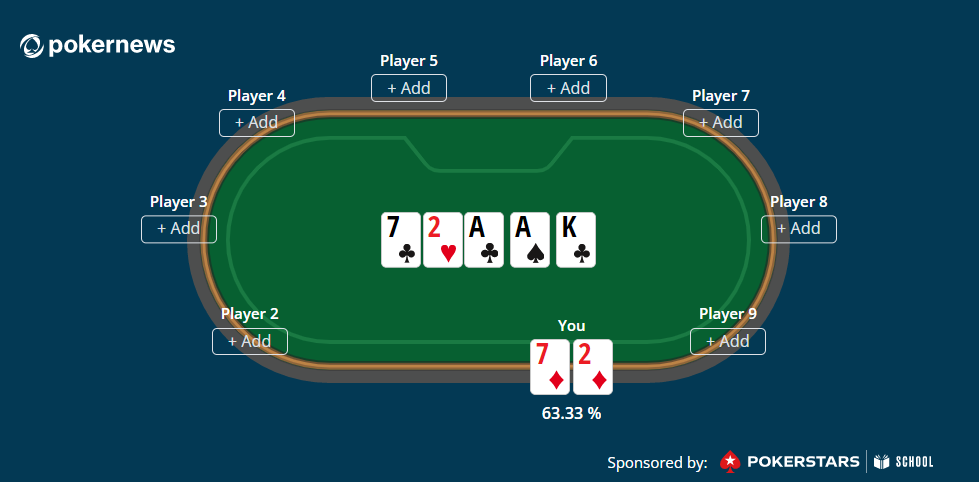
\includegraphics[scale=0.7]{images/test-ps.png}
\caption{A Pokerstars alkalmazásának számítási eredménye river-nél}
\label{fig:test-ps}
\end{figure}

\begin{figure}[h]
\centering
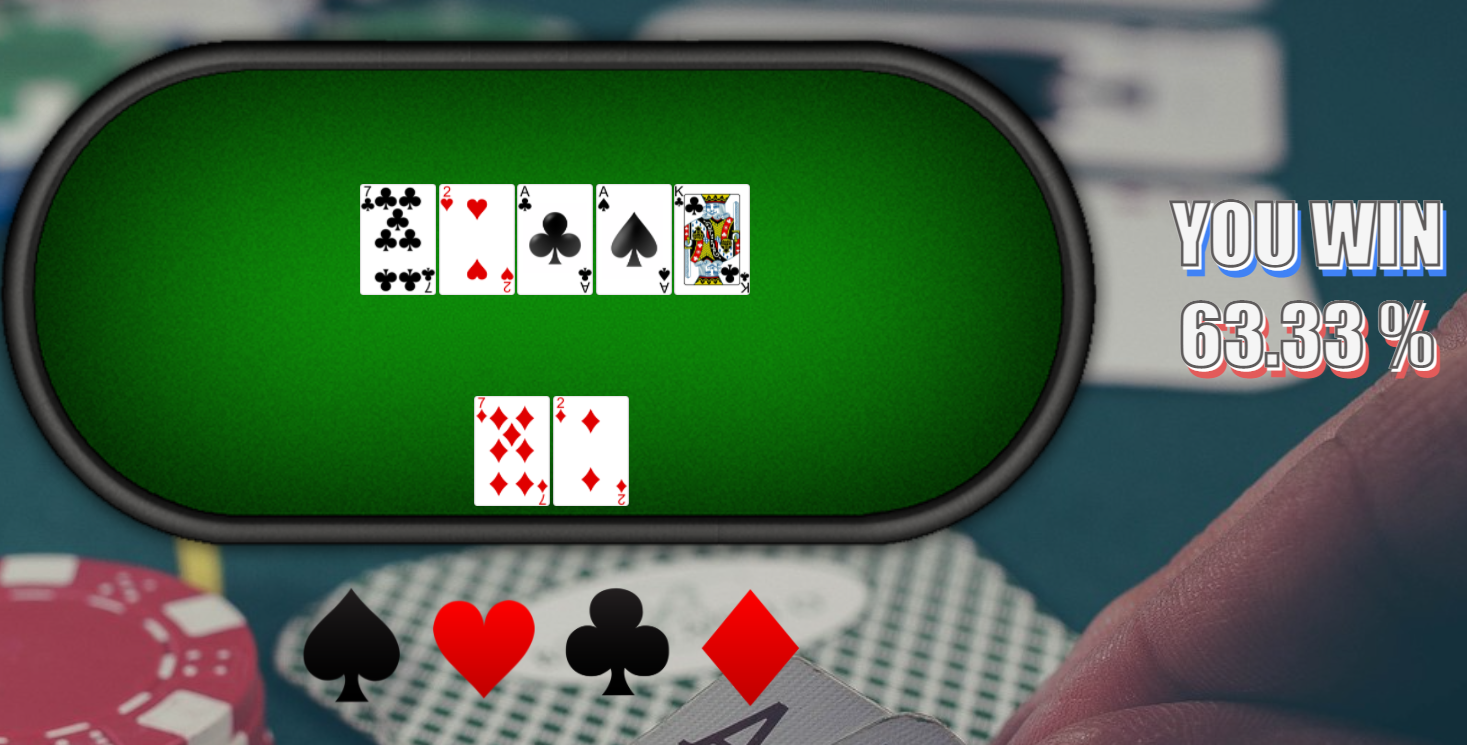
\includegraphics[scale=0.47]{images/test-my.png}
\caption{Az alkalmazásom számítási eredménye river-nél}
\label{fig:test-my}
\end{figure}

\newpage

A diagramm helyes működésének a vizsgálata már bonyolultabb folyamat. Ebben az esetben azt a megoldást választottam, hogy egy olyan kártyakombinációt választok, amelynek viszonylag egyedi diagrammja lesz. Például turn-nél négy treff van az asztalon, a felhasználó kezében két káró van és sem párt, sem erősebb kezet nem alkotnak a lapok. Ebben az estben, ha még egy pikk értkezne river-nél, akkor a board-on lévő lapok flush-t alkotnának, amit a program nyereségként ábrázol. Tehát a diagrammon azt kell látnunk, hogy a maradék pikk lapok esetén nagyon magas a nyerési esélye a felhasználónak.

\begin{figure}[h]
\centering
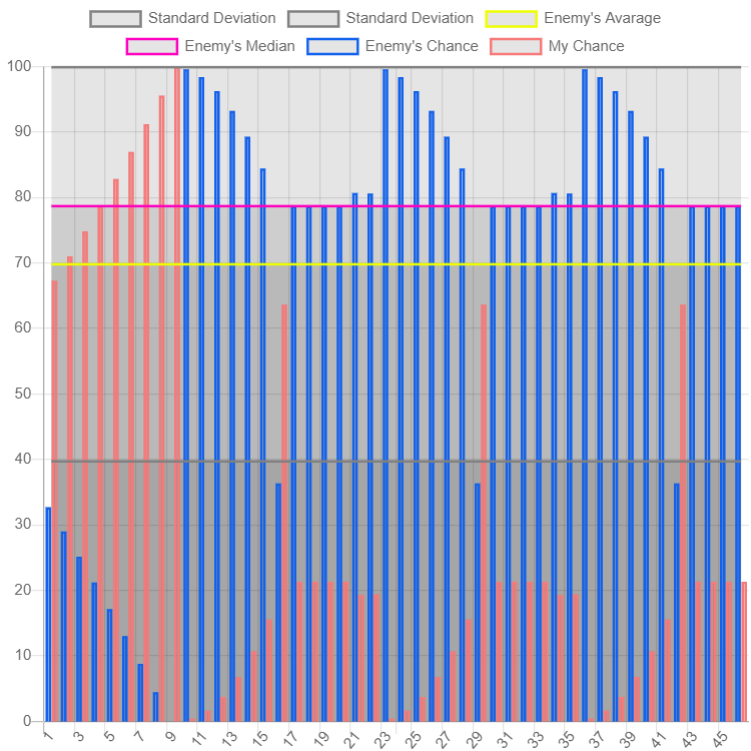
\includegraphics[scale=0.9]{images/chart-test.png}
\caption{A kirajzolt diagramm turn-nél}
\label{fig:chart-test}
\end{figure}

Ennek megfelelően kiválasztottam a felhasználó lapjainak a káró 2-est és 3-mast, az asztalra pedig a treff ászt, királyt, dámát, és bubit. Ezután legeneráltam a diagrammot, ami alább látható. Az everyCards tömbben növekő sorrendben helyezkednek el a lapok, először a treff, majd a káró, kör, végül pedig a pikk. A lapokból az látszik, hogy ha bármelyik treff következik a river-nél, akkor a board-on flush alakulna ki, ha a treff 10-es érkezne, akkor pedig royal flush. Ezen kívül, ha bármilyen 10-es érkezne, akkor sor alakulni ki a boardon, ami szintén a felhasználónak kedvez. A kézben lévő lapok a lehető legalacsonyabbak, illetve nem alakulhat ki belőle flush, sor, de még csak egy drill sem. Ha nem érkezik több treff, akkor a legmagasabb kezünk ami lehet, az egy hármas pár, viszont ez sem mondható erősnek, mivel az asztalon csupa magas lap van. 

Ezeket a tényeket mutatja be a 4.3-as ábrán kirajzolt diagramm. A piros oszlop a felhasználó nyerési esélyeit mutatják, a kékek pedig az ellenfelét. Jól látszik, hogy az első kilenc kártyánál nagyon magas a nyerési esélye a felhasználónak. Ezek a maradék treff lapok a pakliban, az utolsó pedig a treff 10-es, aminél 100\% az esély a győzelemre. A többi lapra három kivétellel mindegyiknél az ellenfélnek nagyobb az esélye. Ez a három lap a maradék 10-esek a pakliban, amelyekkel sor alakulna ki a boardon. A lila konstans mutatja az ellenfél esélyeinek mediánját, a sárga az átlagát, a szürkék pedig a szórását. Ezek mind segítik a felhasználót a döntéshozásban.
% \Chapter{Tesztelés}


\Chapter{Összefoglalás}
Számtalan tapasztalatot szereztem a szakdolgozatom megírása közben. Mivel még nem foglalkoztam webalkalmazás fejlesztéssel, így rengeteg tanulás előzte meg a program elkészítését. Megismerkedtem a Vue JS-el, a Node JS-el, és más nyelvekkel vagy keretrendszerekkel, amiket a szakdolgozatom készítése során felhasználtam. Szerencsére mindegyikük jól dokumentált környezet, így sok segítséget kaptam hozzájuk az interneten. Mivel napjainkban egyre inkább elterjedtek a webes alkalmazások, így remélem a jövőben is hasznomra válnak majd ezek az ismeretek.

Olyan témát sikerült választanom, amely az életben is közel áll hozzám, így nagy lelkesedéssel álltam hozzá az egész munkafolyamathoz. Megtaláltam a párhuzamot a póker és a matematika, statisztika között, amit véleményem szerint sikerült jól megvalósítani és bemutatni. A célomat, hogy egy "csaló programot" hozzak létre, csak megszorításokkal sikerült elérnem. Az alkalmazás tökéletesen megvalósítja az elképzeléseimet, kizárólag a futási idő akadályozó tényező az életben való felhasználásában. Hamar világossá vált számomra, hogy a fejlesztésnek egy nagyon fontos része a tervezés, hiszen az adja a program alapját. Érdekes volt számomra az is, hogy egy olyan alkalmazást sikerült létrehoznom, amelyhez hasonlót világhírű pókerrel foglalkozó társaságok alkottak meg.

A webalkalmazás gyakorlatban való felhasználásra a következők a megállapításaim. Mindenképpen tovább kellene optimalizálni a futási időt, hogy gördülékenyebben lehessen használni. Továbbá hasznos lehet reszponzívvá tenni az alkalmazást, hogy mobilról, táblagépről és más eszközökről is felhasználóbarát megjelenést kapjon. Ha pedig a felhasználók körét szeretnénk bővíteni, akkor az általam használt módszerrel más pókerfajták szimulációját is el lehetne készíteni. Ha csak a Texas Hold'Em-nél maradunk, akkor a fix limit és a pot limit változatát is meg lehetne valósítani, vagy akár az Omaha-t, 5 lapos pókert is.

\clearpage

\addcontentsline{toc}{chapter}{Irodalomjegyzék}
\bibliographystyle{plain}
\bibliography{dolgozat.bib}

\newpage

\pagestyle{empty}

\noindent \textbf{\Large CD Használati útmutató}

\vskip 1cm

A CD gyökerében lévő szakdolgozat jegyzékben két jegyzék található. A dolgozat, és a program jegyzék. 

A dolgozat jegyzékben található a dolgozat LaTeX forráskódja, és a .pdf formátuma is, dolgozat.pdf néven. 

A program jegyzékben található a webalkalmazás forráskódja. 

Fel kell telepíteni a node.js-t, amit a https://nodejs.org/en/ oldalról lehet letölteni.

Node.js telepítése után, a parancssorban a következő utasítást kiadva: \texttt{npm install vue} feltelepül a Vue.js keretrendszer.


Miután elkészültünk ezekkel, a program jegyzékben találunk egy frontend és egy backend jegyzéket. Mind a két jegyzékben ki kell adni az alábbi parancsokat: 
\begin{itemize}
    \item \texttt{npm install}
    \item \texttt{npm run serve}
\end{itemize}


A frontend jegyzék parancssorában megjelenő ://Localhost címen fogjuk elérni a programot a böngészőnkből.


\end{document}
